\documentclass[11pt]{article}
\usepackage{graphicx}
\usepackage[margin=2.5cm]{geometry}
\usepackage{tikz}
\usepackage{indentfirst}
\usepackage{tabularx}
\usepackage{listingsutf8}
\usepackage{color}
\usepackage{titlesec}
\usepackage{multirow}
\usepackage{adjustbox}
\usepackage[portuguese]{babel}

\setcounter{secnumdepth}{4}

\graphicspath{{./images/}}

\def\checkmark{\tikz\fill[scale=0.4](0,.35) -- (.25,0) -- (1,.7) -- (.25,.15) -- cycle;} 
\setlength{\parskip}{0.5em}

\lstset{
	belowcaptionskip=1\baselineskip,
	captionpos=b,
	frame=tb,
	language=C,
	aboveskip=3mm,
	belowskip=3mm,
	showstringspaces=false,
	columns=flexible,
	basicstyle={\small\ttfamily},
	numbers=none,
	numberstyle=\tiny\color{gray},
	keywordstyle=\color{blue},
	commentstyle=\color{dkgreen},
	stringstyle=\color{mauve},
	breaklines=true,
	breakatwhitespace=true,
	tabsize=3,
	inputencoding=utf8,
	extendedchars=true,
	literate={á}{{\'a}}1 {ã}{{\~a}}1 {à}{{\`a} }1 {Ã}{{\~A}}1 {ó}{{\'o}}1 {Ó}{{\'O}}1 {Í}{{\'I}}1 {í}{{\'i}}1 {é}{{\'e}}1 {ç}{{\c{c}}}1 {Ç}{{\c{C}}}1 {ú}{{\'u}}1
}

\begin{document}
	\begin{titlepage}
	\begin{center}
		
		
\includegraphics[width=0.3\textwidth]{logo-isec}
		
		\normalsize
		Licenciatura em Engenharia Informática - Curso Europeu \\
		28 de maio de 2021
		
		\LARGE
		Gestão - 2020/2021
		
		\large
		Doutor Jorge Alexandre Almeida
		
		\vspace{1.5cm}
		
		
\includegraphics[width=0.3\textwidth]{logo}

		\vspace{0.5cm}

		\Huge
		\textbf{AquiTerrenos, Lda}
		
		\LARGE
		\textbf{Plano de Negócios}
		
		\vspace*{\fill}
		
		\Large
		
		\begin{tabular}{ccc}
			\textbf{Sofia Janeiro} & \textbf{José Almeida} & \textbf{Rúben Lousada} \\ 
			2019132578 & 2019129077 & 2019126176 \\
		\end{tabular}
	
		\vspace{.5cm}
		
		\vfill
		\vspace*{\fill}
		
		
	\end{center}
\end{titlepage}
	
	\tableofcontents
	\pagebreak
	
	\large
	\section{Sumário Executivo}
	
	\normalsize
	
	Possuir e manter terrenos é algo que faz parte da vida de muitos indivíduos e famílias. Por vezes, por falta de visão geral e/ou de conhecimento acerca dos próprios terrenos que possuem, podem-se gerar desentendimentos e dificuldades na sua localização. Com o crescimento da literacia informática da população, faz todo o sentido a procura da informatização do seu património. Muitas vezes, os proprietários dos terrenos procuram fazê-lo, mas não encontram uma solução viável e simples.
	
	A AquiTerrenos pretende resolver esse problema: tem como finalidade servir como uma pequena base de dados para cada família ou indivíduo, onde pode guardar toda a informação que achar relevante sobre os seus terrenos (como pinhais, eucaliptais, vinhas, etc.), assim como partilhar o acesso à mesma com quem quiser, facilitando o acesso a outros serviços externos.
	
	O nosso objetivo é dar ao cliente uma visão alargada sobre os seus terrenos, que o permita gerir os mesmos da forma mais eficiente possível, assim como partilhar informações dos mesmos à sua família / amigos / cooperativas agrícolas, de modo a fomentar e facilitar a cooperação entre proprietários. Implementaremos funcionalidades como geolocalização, informações topográficas, do solo, da fauna e da flora, visualização 3D e 360ª do terreno, entre outras.
	
	Para tirar o máximo proveito dessas funcionalidades, a AquiTerrenos funcionará também como um mercado de terrenos, que irá usar as informações já inseridas pelo cliente sobre os seus terrenos, caso este queira vender os mesmos. Isto simplifica o processo de venda para utilizadores da funcionalidade descrita nos parágrafos anteriores, pois, num caso ideal, já não será necessária a inserção de informação adicional sobre os terrenos que pretende vender, algo que fará com que o utilizador seja mais propício a usar o mercado da AquiTerrenos, e não qualquer outro.
	
	Esta proposta de solução tem de ser rentável para a empresa. Assim, surge a ideia de criação de uma aplicação, inicialmente grátis, onde possa ser feita essa gestão dos terrenos, assim como interagir com o mercado. Algumas funcionalidades estarão barradas por um pagamento único, outras estarão associadas a subscrições mensais/anuais.
	
	A partir de um pequeno estudo de mercado, observamos que por volta de 25\% das famílias que participaram desse estudo não possuem um registo (em papel ou informatizado) dos terrenos que possuem. Este seria o público-alvo do nosso serviço. Além disso, 90\% reportou interesse em utilizar a nossa aplicação e o mercado associado.
	
	De momento, a empresa encontra-se num estado teórico, sendo o próximo passo o desenvolvimento de um protótipo de modo a estudar ainda mais o mercado e o nosso público alvo. Estimamos que, no fim de um período de 5 anos, teremos um VAL de 1.700.000€, assim como uma TIR de aproximadamente 116\%. Estimamos, também, a recuperação do investimento inicial em 4 anos.
	
	\pagebreak
	
	\large
	\section{Apresentação do Negócio}
	\subsection{Identificação da Empresa}
	
	\normalsize
	
	\begin{center}
		\begin{tabular}{ | l | r | }
			\hline
			Designação Social: & AquiTerrenos, Lda \\
			\hline
			Nº de Contribuinte: & 001122334 \\
			\hline 
			Distrito: & Coimbra \\
			\hline   
			Concelho: & Coimbra \\
			\hline   
			Localidade: & Coimbra \\
			\hline   
			Morada (Sede Social): & Rua Pedro Nunes \\
			\hline   
			Telefone: & 123 456 789 \\
			\hline 
			Fax: & 123 456 789 \\
			\hline 
			URL: & aquiterrenos.com \\
			\hline
			E-mail: & aquiterrenosgeral@gmail.com \\
			\hline 
			Responsável: & José Almeida \\
			\hline 
			Cargo: & CEO \\ 
			\hline
			Móvel: & 123 456 789 \\
			\hline 
			Fax: & 123 456 789 \\
			\hline 
			E-Mail: & a2019129077@isec.pt \\
			\hline 
			Data de Constituição e Inicio da Atividade: & 01-06-2021 \\
			\hline 
			Forma Jurídica: & Sociedade por Quotas \\
			\hline 
			Capital Social: & 3.000€ \\
			\hline
			\multirow{3}{*}{Principais Accionistas:} & José Almeida \\
			& Rúben Lousada  \\
			& Sofia Janeiro  \\
			\hline 
			CAE: & 58290 \\
			\hline 
		\end{tabular}
	\end{center}

	\large
	\subsection{Denominação e Forma Jurídica Adotadas}
	
	\normalsize
	
	A denominação "AquiTerrenos, Lda" permite identificar, de forma distintiva e fácil de memorizar, a empresa. Apesar de não ser um nome adequado à internacionalização, consideramos que a designação escolhida, por estar em português, é ideal para ganhar força no mercado nacional. Posteriormente, terá de ser adaptado a cada país em que a empresa operar.
	
	Pretende-se que a empresa tome a forma jurídica de sociedade por quotas, devido às vantagens provenientes da mesma, nomeadamente a limitada responsabilidade dos sócios ser limitada aos bens afetos à empresa, tendo isso como consequência o baixo risco pessoal dos sócios.
	
	Outra vantagem clara é o baixo capital social necessário à criação da empresa, o que permite o desenvolvimento inicial da solução apresentada sem grande investimento necessário da parte dos sócios.
	
	Inicialmente, a empresa teria 3 sócios, sendo estes também os autores deste documento.
	
	\pagebreak
	
	\large
	\subsection{Historial da Empresa}
	
	\normalsize
	
	Tendo sido identificadas deficiências a nível de gestão e conhecimento das propriedades, a AquiTerrenos surge como possível solução aos mesmos. Tem como objetivo ajudar os clientes na gestão e conhecimento sobre as suas propriedades, tirando, assim, um maior proveito das mesmas. Esperamos crescer a uma escala não só nacional, como também internacional. A empresa será fundada como uma start-up, em Coimbra, por alunos de Engenharia Informática.
	
	A empresa procurará conceber, desenvolver e comercializar uma aplicação para smartphone, que terá, simultaneamente, características de produto e características de serviço. Esta aplicação terá, também, secções destinadas ao comércio online, ou seja, eCommerce.
	
	A nossa equipa é, atualmente, composta por três elementos. Sendo estes estudantes de Informática, a nossa equipa tem as competências necessárias à criação e gestão da solução proposta, por se tratar de uma aplicação. Toda a equipa tem, também, conhecimentos de inglês a níveis fluentes, assim como alguns conhecimentos de alemão e francês.
	
	\vspace{1cm}
	
	\begin{figure}[h]
		
\includegraphics[width=0.15\textwidth,keepaspectratio]{jalmeida}
		\label{fig:ja}
		\centering
	\end{figure}
	
	\vspace{0.3cm}
	
	José Almeida nasceu em Coimbra e viveu sempre em Miranda do Corvo. Concluiu os seus estudos secundários no Curso de Ciêcnais e Tecnologia. É agora estudante na Licenciatura de Engenharia Informática - Curso Europeu. Destaca-se pela suas qualidades de liderança e conhecimentos de informática. É fluente em inglês e tem alguns conhecimentos de alemão.
	
	\vspace{1cm}
	
	\begin{figure}[h]
		
\includegraphics[width=0.15\textwidth,keepaspectratio]{rlousada}
		\label{fig:rl}
		\centering
	\end{figure}
	
	\vspace{0.3cm}
	
	Nascido em Viseu, Rúben viveu desde pequeno em Aveiro, onde efetuou todo o seu percurso escolar até ao 12º ano. No secundário, frequentou o Curso Profissional de Programação e Gestão de Sistemas Informáticos. Estuda, agora, no Instituto Superior de Engenharia de Coimbra, na Licenciatura de Engenharia Informática - Curso Europeu. Destaca-se ainda mais pelos seus conhecimentos de informática, tendo mais experiência do que o resto da equipa. É fluente em inglês e tem alguns conhecimentos de alemão.
	
	\vspace{1cm}
	
	\begin{figure}[h]
		
\includegraphics[width=0.15\textwidth,keepaspectratio]{sjaneiro}
		\label{fig:sj}
		\centering
	\end{figure}
	
	\pagebreak
	
	Sofia viveu, desde sempre, em Coimbra onde concluiu os seus estudos secundários no Curso de Ciências e Tecnologias. Atualmente, estuda no Instituto Superior de Engenharia de Coimbra em Engenharia Informática (Curso Europeu). Destaca-se na equipa devido às suas capacidades de design, sendo importantíssima para a imagem da empresa. É fluente em inglês e tem alguns conhecimentos de francês.
	
	\vspace{1cm}
	
	\large
	\subsection{Visão}
	
	\normalsize
	
	A AquiTerrenos pretende, no futuro, ser líder na área de ajuda à manutenção e gestão de propriedades. Tem como objetivo estar presente em todo o mundo e, assim, facilitar a gestão de terrenos possuídos, quer sejam por pessoas ou empresas a uma escala global.
	
	Acreditamos que uma frase que descreve bem a nossa visão é "Poder sobre o que é seu", pois o objetivo da empresa, a um nível geral, é esse mesmo: dar conhecimento (e, consequentemente, poder) aos proprietários sobre aquilo que possuem.
	
	\large
	\subsection{Missão}
	
	\normalsize
	
	Através de uma aplicação para smartphone, pretendemos dar ao cliente possibilidades de melhorar a qualidade e diminuir o tempo necessário à gestão das suas propriedades.
	
	Através de diversos planos de pagamento na aplicação, pretendemos oferecer aos nossos stakeholders um investimento bastante positivo, quer em termos monetários, no caso dos investidores, quer em termos de tempo despendido, no caso de outros colaboradores.
	
	A empresa pretende oferecer planos de baixo custo, de modo a poder expandir ao máximo o acesso aos nossos produtos e serviços, crescendo o negócio e procurando alcançar, da melhor forma possível, a nossa visão.
	
	\large
	\subsection{Vetores Estratégicos}
	
	\normalsize
	
	De modo a garantir o bem-estar da empresa e o cumprimento dos objetivos já referenciados, é necessário formular uma estratégia empresarial clara.
	
	A AquiTerrenos não prevê necessidade de investir em I\&D, pois esta, tratando-se de uma startup de capacidades reduzidas, deve focar-se no desenvolvimento e manutenção da solução de mercado proposta.
	
	Inicialmente, a empresa não necessitará de uma secção de RH altamente qualificada e, como tal, deve poupar nesse aspeto, até esta ser necessária (nomeadamente durante a internacionalização, devido ao aumento do número de colaboradores necessários).
	
	Serão estabelecidas parcerias com imobiliárias, que poderão guardar no nosso sistema os terrenos dos quais estão encarregues, e/ou vender os mesmos no nosso mercado intergrado. Será também estudada a possibilidade de fazer parcerias com governos de países, de modo a poder interligar e verificar, com a ajuda de uma fonte oficial, a informação inserida pelos clientes.
	
	\large
	\subsection{Localização das Instalações e Descrição do Local}
	
	\normalsize
	
	Relativamente à localização das instalações, o principal objetivo seria conseguir um lugar na incubadora IPN, na Rua Pedro Nunes, em Coimbra, sendo essa a sede da nossa start-up. Caso isso não seja possível, tentaremos obter lugar noutras incubadoras, nomeadamente o INOPOL. Caso isso se revele igualmente impossível, desenvolveremos o produto remotamente e, no segundo ano de vida da empresa, será arrendado um escritório em Coimbra.
	
	\large
	\subsection{Razões para a escolha da localização}
	
	\normalsize
	
	A razão de escolha de incubadoras como o IPN e o INOPOL é clara. Tratando-se a empresa de uma start-up na área de software, estas são uma excelente fonte de colaboradores, assim como de ajuda a níveis legais, económicos e de desenvolvimento, algo que será muito importante obter para garantir o sucesso da empresa, pois a nossa equipa, apesar de ter conhecimentos de informática, não tem altos conhecimentos nas áreas acima referidas. 
	
	A localização destas ajudará, também, na procura de talentosos jovens colaboradores, que tenham feito o seu percurso académico em Coimbra ou nas redondezas.
	
	Em último caso, será arrendado um escritório em Coimbra pela mesma razão disposta no parágrafo anterior, mas também pelos custos reduzidos comparados a arrendar um escritório e ter sede em Lisboa ou no Porto.
	
	\pagebreak
	
	\large
	\section{Análise do Produto/Serviço}
	
	\normalsize
	
	\large
	\subsection{Descrição Sumária dos Serviços}
	
	\normalsize
	
	\begin{center}
		\begin{tabularx}{\linewidth}{ | p{0.2\textwidth} | X | }
			\hline
			\multirow{3}{*}{Plano Base} & Plano inicial simples, permitindo o acesso apenas a funcionalidades essenciais, como adicionar terrenos e partilhar os mesmos com outros utilizadores, ou ver a topografia dos mesmos. \\
			\hline
			\multirow{4}{*}{Plano Lifetime} & Plano de compra única cujo objetivo é meramente expandir as funcionalidades da versão grátis da aplicação, sem adicionar novas. Por exemplo, aumentar o limite de terrenos que se podem guardar simulaneamente por cliente. \\
			\hline
			Plano Subscrição 1: Anúncios no Mercado & Plano de subscrição mensal ou anual que permite manter mais que um anúncio simultaneamente no mercado, assim como dar boost gratuitamente a um anúncio. \\
			\hline 
			Plano Subscrição 2: Suporte a Terrenos Cultivados & Plano de subscrição mensal ou anual que visa dar suporte a terrenos cultivados, contendo informação útil para esse efeito como, por exemplo, o estado do cultivo e algumas recomendações. \\
			\hline   
			\multirow{2}{*}{Plano Premium} & Plano de subscrição mensal ou anual que inclui todos os planos anteriores, expandindo-os e disponibilizando também novas funcionalidades.  \\
			\hline
		\end{tabularx}
	\end{center}
	
	\large
	\subsection{Vantagens Distintivas}
	
	\normalsize
	
	\begin{center}
		\begin{tabularx}{\linewidth}{ | p{0.2\textwidth} | X | }
			\hline
			\multirow{4}{*}{Plano Base} & Distingue-se da concorrência pois proporciona uma maneira fácil de guardar alguns dos terrenos, sem qualquer pagamento associado. Também é único devido à possibilidade de partilhar a informação sobre os terrenos com outros utilizadores. \\
			\hline
			\multirow{2}{*}{Plano Lifetime} & Dinstingue-se da concorrência devido ao seu baixo custo e duração ilimitada. \\
			\hline
			\multirow{4}{=}{Plano Subscrição 1: Anúncios no Mercado} & Distingue-se dos concorrentes pois permite que os utilizadores mais intensivos da aplicação, que nela já têm os seus terrenos guardados, possam colocar à venda um número indeterminado das suas propriedades possuindo esta subscrição. \\
			\hline 
			Plano Subscrição 2: Suporte a Terrenos Cultivados & Distingue-se da concorrência devido ao suporte muito útil que fornece ao utilizador, mantendo-o a par da situação das suas propriedades. \\
			\hline   
			\multirow{2}{*}{Plano Premium} & Distingue-se da concorrência pelas razões acima apresentadas, pois inclui todos os outros planos.  \\
			\hline
		\end{tabularx}
	\end{center}
	
	
	\large
	\subsection{Desenvolvimentos Previsíveis dos Serviços}
	
	\normalsize
	
	A médio/longo prazo, pretendemos alargar a gama de funcionalidades disponíveis na nossa aplicação. O conteúdo dessas funcionalidades será decidido tendo um contacto direto com os utilizadores da nossa solução, através de inquéritos e / ou entrevistas aos mesmos. Procurar-se-á sempre melhorar o design e a eficácia do serviço.
	
	
	\large
	\subsection{Tecnologias a Utilizar e Direitos da Propriedade Industrial}
	
	\normalsize
	
	As tecnologias necessárias ao desenvolvimento da nossa aplicação serão, preferencialmente, de código aberto, permitindo o uso das mesmas sem grandes custos.
	
	No entanto, há certos serviços como, por exemplo, o Google Maps, que, para serem implementados na nossa aplicação, necessitarão de licenças, que não prevemos serem caras ou difíceis de obter.
	
	
	\large
	\subsection{Processo Produtivo}
	
	\normalsize
	
	Tratando-se de uma aplicação para smartphone, depois do desenvolvimento a mesma será colocada nas lojas conhecidas, tais como o Google Play Store e o App Store. O cliente, depois de se registar na nossa aplicação, poderá imediatamente usufruir dos benefícios do plano base. Se assim desejar, poderá comprar/subscrever a qualquer um dos outros planos através de pagamento eletrónico.
	
	
	\large
	\subsection{Layout das instalações}
	
	\normalsize
	
	Tratando-se a AquiTerrenos, Lda de uma start-up, inicialmente as instalações serão simples e devem ser, durante todo o tempo de existência da empresa, adequado ao número de colaboradores da mesma. Deverá estar organizada em zonas, especialmente as 4 seguintes: Manutenção, Marketing, Desenvolvimento e Recursos Humanos. Em princípio, devido à natureza do projeto, não necessitará de uma zona de atendimento ao cliente. No entanto, deverá incluir uma zona de lazer e, naturalmente, salas de conferência.
	
	\vspace{1cm}
	
	\begin{figure}[h]
		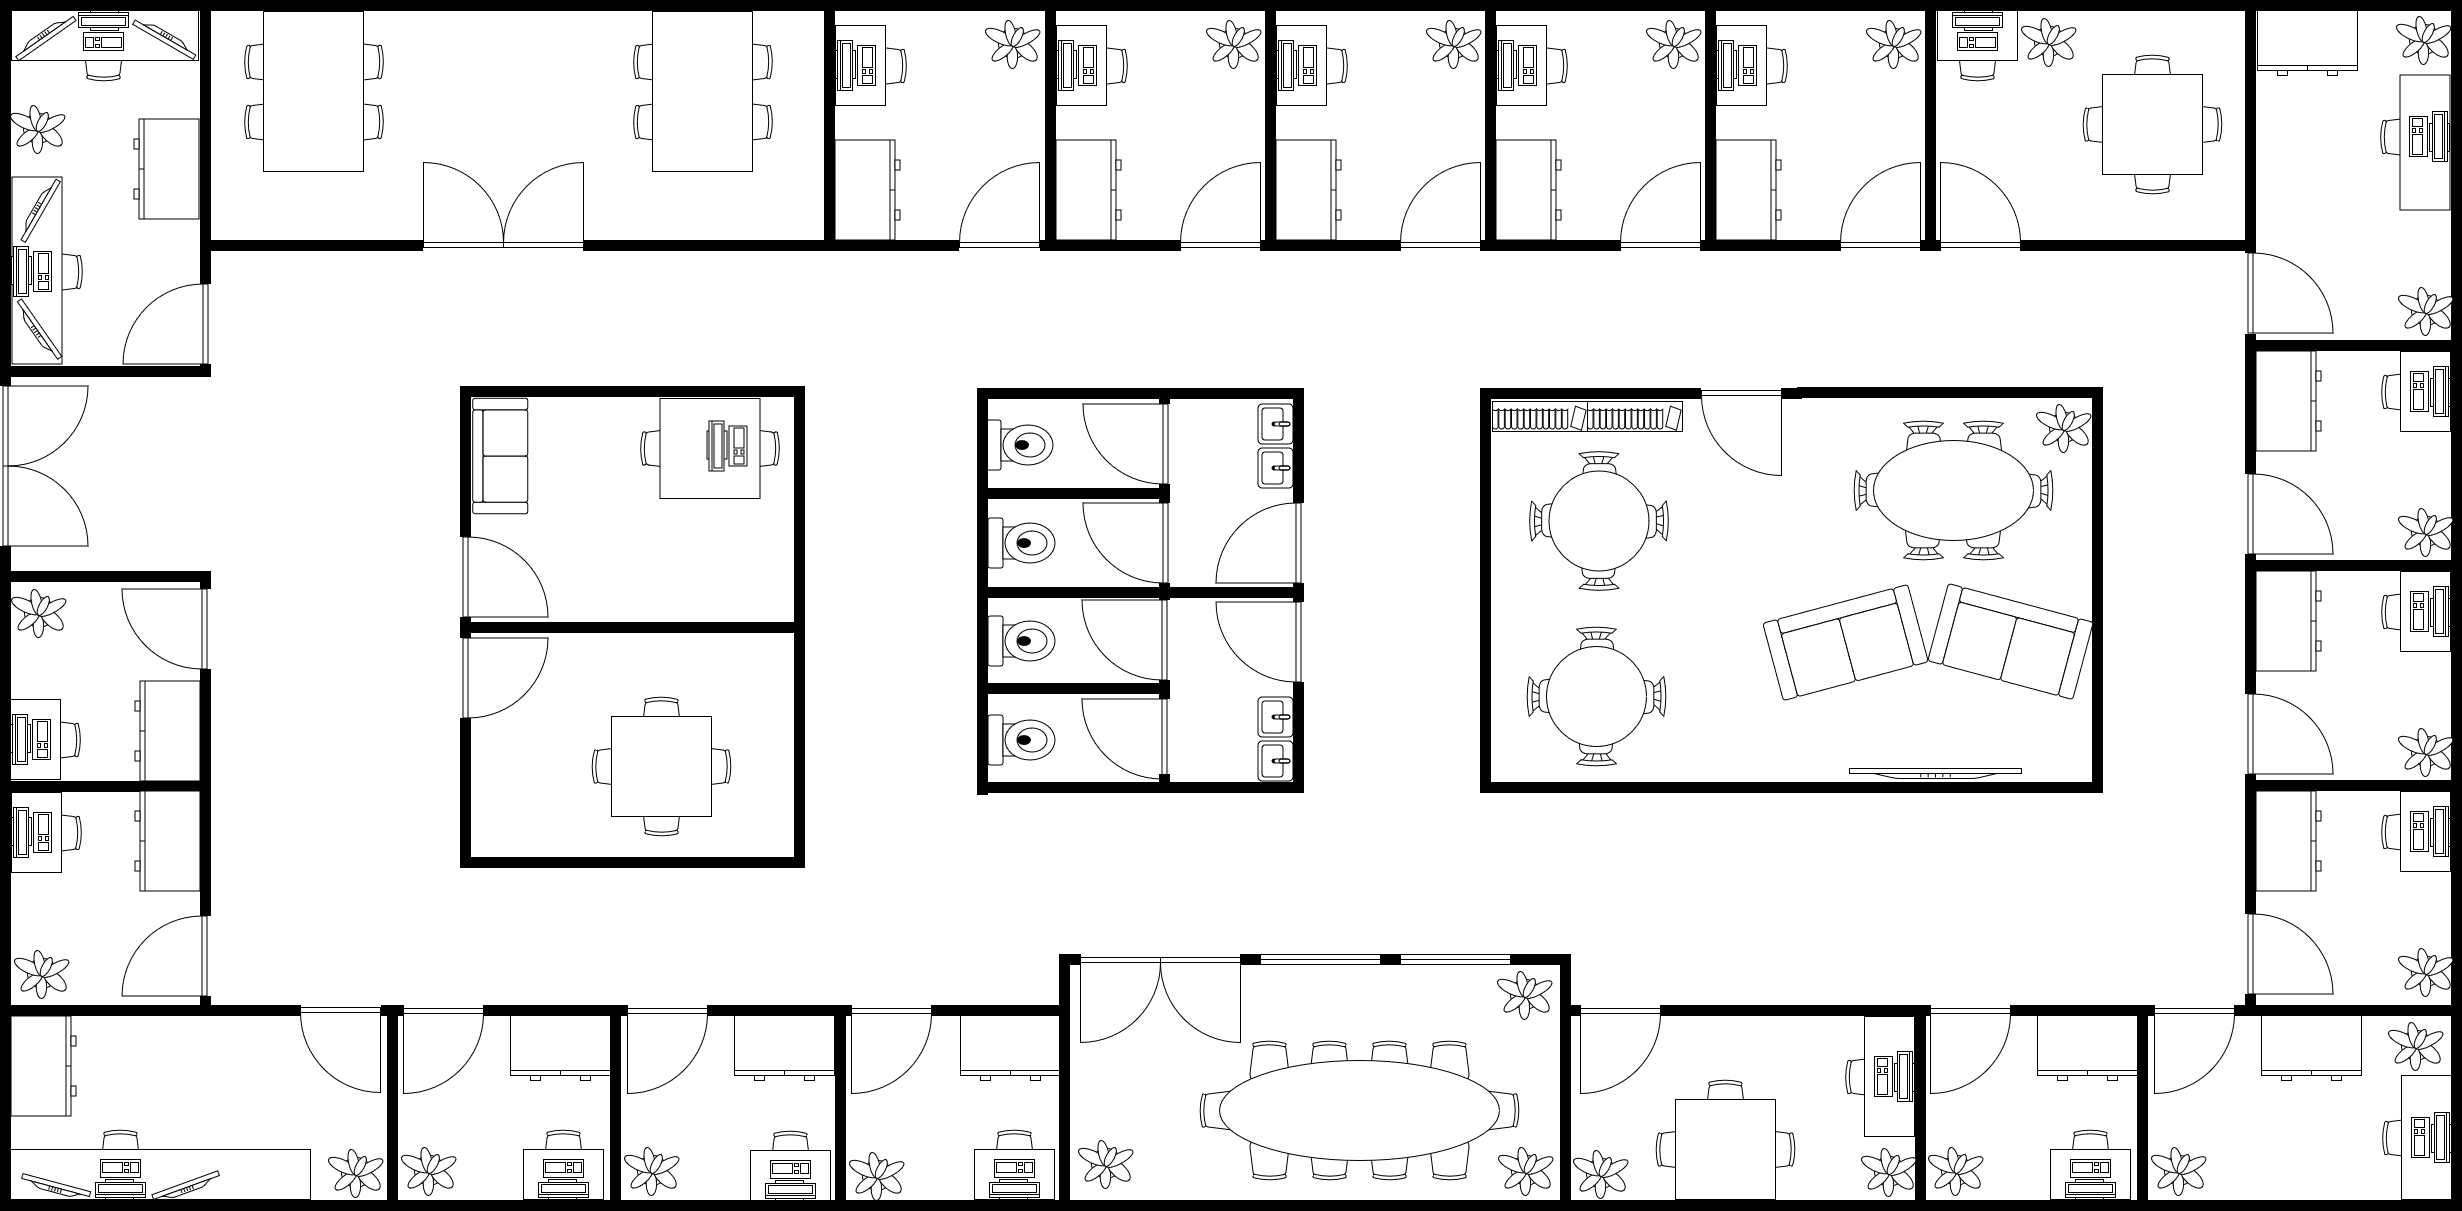
\includegraphics[width=0.9\textwidth,keepaspectratio]{planta}
		\label{fig:planta}
		\centering
		\caption{Planta das Instalações}
	\end{figure}
	
	\pagebreak
	
	\large
	\section{Análise de Mercado}
	
	\normalsize
	
	\large
	\subsection{Evolução Histórica e Previsional do Setor (Problemas e Tendências)}
	
	\normalsize
	
	Com a solução apresentada, pretendemos nos inserir no sector de software imobiliário para efeitos rurais, através da prestação de serviços (SaaS). O modelo SaaS tem vindo a crescer ao longo dos anos, com previsões para continuar esse crescimento, à medida que cada vez mais pessoas possuem um smartphone e os níveis de literacia informática aumentam. Devido a esse crescimento na procura, espera-se também um crescimento contínuo da oferta, nascendo cada vez mais empresas que utilizam esse modelo de negócio. 
	
	Um grande problema de serviços em zonas mais rurais é o acesso às mesmas, pois muitas vezes não compensa uma empresa se deslocar para essas zonas e fornecer os seus serviços.
	
	\begin{figure}[h]
		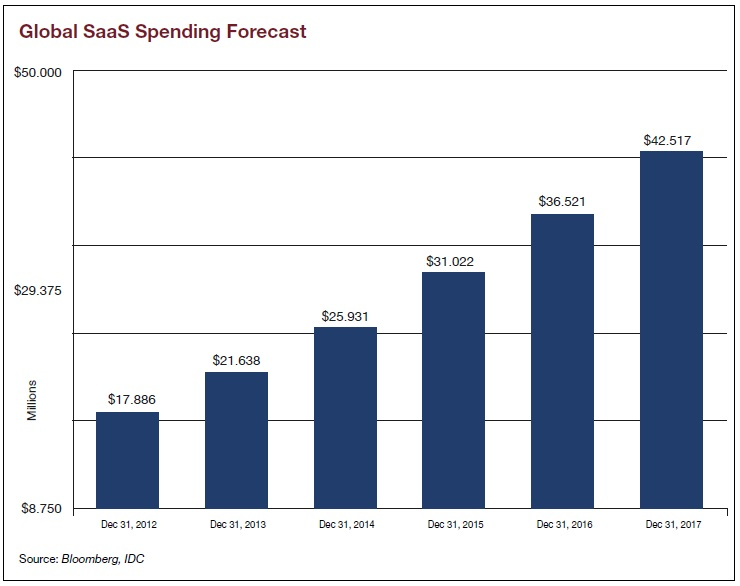
\includegraphics[width=0.6\textwidth,keepaspectratio]{crescimentoSaaS}
		\label{fig:crescimentoSaaS}
		\centering
		\caption{Crescimento do Modelo SaaS}
	\end{figure}
	
	
	
	\large
	\subsection{Enquadramento do Negócio no Setor}
	
	\normalsize
	
	O nosso negócio pretende responder a esta necessidade crescente de produtos de software no mercado imobiliário rural, procurando atingir um público que, até aos dias de hoje, não teve muita representação a esse nível, devido aos seus reduzidos conhecimentos de informática (pois muitas vezes os proprietários de terras são, por exemplo, de idade avançada e sem smartphone), algo que está de dia para dia a mudar.
	
	Usando a nossa solução de negócio o modelo SaaS, poderá, através do uso autónomo da mesma por parte dos utilizadores, alcançar todas as zonas rurais do mundo, desde que exista um acesso à Internet nas mesmas.
	
	
	\large
	\subsection{Caracterização do Mercado Alvo}
	
	\normalsize
	
	Atendendo a um pequeno estudo de mercado que efetuamos, cerca de 80\% dos indivíduos e família em primeiro e segundo grau (filhos, pais e avós) possuem pelo menos um terreno (sem construções). Para além disso, 63\% desses participantes afirmaram não conhecer todos os limites dos seus ou dos terrenos da sua família.
	
	Considerando que existem cerca de 500.000 desses conjuntos de pessoas em Portugal, podemos considerar que o número de potenciais clientes é de 63\% de 400.000, ou seja, aproximadamente 250.000. Se considerarmos toda a Europa, e usando a mesma estatística de 80\% e 63\%, temos um número de potenciais clientes de cerca de 19.000.000 (embora esse número tenha uma grande margem de erro, devido à natureza do nosso estudo de mercado). Considerando que 5\% das pessoas afetadas por esse problema seriam clientes da nossa aplicação (12.500 em Portugal, 950.000 na Europa) e que, em média, 40\% dos utilizadores do nosso serviço gastariam dinheiro com ele (5.000 em Portugal, 380.000 na Europa), e ainda considerando uma média de 30€/ano de gastos por cliente, temos, por ano, uma receita de 150.000€ em Portugal, ou 11.400.000€, na Europa.
	
	Consideramos que os clientes vão comprar o nosso serviço, pois este satisfará bem a necessidade destes guardarem um registo informático das suas posses, a um preço reduzido.
	
	
	\large
	\subsection{Análise da Concorrência}
	\subsubsection{Identificação}
	
	\normalsize
	
	\begin{center}
		\begin{tabular}{ | c | c | c | }
			\hline
			& Nacional & Internacional \\
			\hline
			Plano Base & BUPi & Provas de Conceito (PoC) \\
			\hline
			Plano Lifetime & BUPi & Provas de Conceito (PoC) \\
			\hline
			Plano Subscrição 1: Anúncios no Mercado & Imobiliárias & Imobiliárias \\
			\hline 
			Plano Subscrição 2: Suporte a Terrenos Cultivados & - & Croptracker \\
			\hline   
			Plano Premium & - & - \\
			\hline
		\end{tabular}
	\end{center}

	\pagebreak
	
	\large
	\subsubsection{Avaliação da Empresa com os seus Principais Concorrentes}
	\normalsize
	
	\begin{center}
		\begin{tabularx}{\linewidth}{ | c | c | X | }
			\hline
			& +/0/- & Porquê \\
			\hline
			\multirow{3}{*}{Gama de Produtos / Serviços} & \multirow{3}{*}{+} & Os concorrentes apenas oferecem soluções para um dos problemas referidos, enquanto a AquiTerrenos oferece solução para vários deles. \\
			\hline
			\multirow{2}{*}{Qualidade dos Serviços} & \multirow{2}{*}{+} & A nossa aplicação estará no topo em relação à qualidade de software. \\
			\hline
			\multirow{2}{*}{Serviços Complementares} & \multirow{2}{*}{0} & A AquiTerrenos terá apoio ao cliente, tal como os seus concorrentes. \\
			\hline 
			\multirow{2}{*}{Dimensão} & \multirow{2}{*}{-} & Tratando-se a AquiTerrenos de uma start-up, esta tem dimensão bastante reduzida. \\
			\hline   
			\multirow{2}{*}{Notoriedade} & \multirow{2}{*}{-} & Como a AquiTerrenos não está, de momento, no mercado, esta não tem qualquer notoriedade. \\
			\hline
			\multirow{2}{*}{Imagem} & \multirow{2}{*}{-} & Como a AquiTerrenos não está, de momento, no mercado, este não formou qualquer imagem da mesma. \\
			\hline
			\multirow{2}{*}{Preço} & \multirow{2}{*}{+} & Um dos objetivos da AquiTerrenos é fornecer planos de baixo custo e de qualidade. \\
			\hline
			\multirow{3}{*}{Rapidez de Execução} & \multirow{3}{*}{+} & Tratando-se a nossa solução de uma aplicação totalmente controlada pelo utilizador, esta é tão rápida quanto o próprio utilizador. \\
			\hline
			\multirow{3}{*}{Garantias} & \multirow{3}{*}{+} & A AquiTerrenos oferece garantias de proteção da privacidade de dados dos clientes, assim como estabilidade do serviço. \\
			\hline
		\end{tabularx}
	\end{center}
	
	
	\large
	\subsection{Fornecedores}
	
	\normalsize
	
	Tratando-se de uma empresa cujo modelo de negócio passa por uma solução SaaS, a totalidade dos fornecedores são os fornecedores dos FSE, ou seja, fornecedores de coisas como eletricidade, água e material de escritório. No entanto, há um fornecedor bastante relevante: a empresa que tratará do hosting dos servidores necessários à nossa aplicação. Esta deve oferecer garantias de funcionamento constante do mesmo, sem problemas de rapidez.
	
	\pagebreak
	
	\large
	\section{Estratégia de Marketing}
	\subsection{Segmentação}
	
	\normalsize
	
	Tratando-se a nossa solução de uma aplicação, o seu mercado alvo será, em geral, a população abaixo dos 50 anos, pois possuem mais conhecimentos de informática e, como tal, serão mais propícios de utilizar a nossa aplicação. No entanto, tambén não poderá ser voltada para a população muito jovem (abaixo dos 30 anos), pois estes não possuem, geralmente, terrenos, embora possam recomendar a nossa aplicação para pessoas no seu círculo social. Sendo assim, a faixa etária que esperemos que mais dê uso à nossa solução é a faixa etária entre os 30 e os 50 anos. Tanto homens quanto mulheres possuem e gerem terrenos, pelo que não faz sentido fazer a segmentação do mercado por sexo.
	
	Quanto à segmentação geográfica, entendemos que deve ser feita, pois consideramos que a nossa solução se adapte melhor a um contexto rural do que propriamente a um urbano. Sendo o nosso objetivo oferecer planos de baixo custo, não vemos motivo para fazermos qualquer segmentação a nível de poder de compra.
	
	\large
	\subsection{Política do Produto/Serviço}
	
	\normalsize
	
	Quanto às características do produto, pretendemos que este seja simples de utilizar, sendo esse um dos pontos importantes a passar com a nossa política de marketing. A aplicação deve ser intuitiva, com um foco especial na simplicidade de design e com indicações claras sobre como usar as funcionalidades. Queremos que a imagem de marca da aplicação seja exatamente essa, pois o primeiro contacto físico do cliente com a nossa empresa será através dessa aplicação, tornando a qualidade do design especialmente importante.
	
	De momento, a nossa solução encontra-se num estado ainda teórico, estando definidas linhas e funcionalidades gerais para o desenvolvimento da solução, mas não tendo ainda passado para o nível tecnológico do desenvolvimento. Inicialmente, será desenvolvido um protótipo, com funcionalidades básicas essenciais à aplicação. Deve ser recolhida o máximo de informação sobre a user experience desse protótipo, que será tomada em conta ao longo do desenvolvimento da aplicação completa. Ao longo do ciclo de vida do serviço, serão continuamente feitos inquéritos aos utilizadores, de modo a poder adaptar o mesmo ao cliente, procurando assim aumentar o seu sucesso.
	
	\pagebreak
	
	\large
	\subsection{O Preço}
	
	\normalsize
	
	Sendo a nossa solução uma aplicação, esta possui uma elevada margem de lucro, pois a maior parte do seu custo está no desenvolvimento e manutenção da mesma. Sendo assim, podem ser aplicados preços mais baixos, com o objetivo de aumentar o número de vendas. No entanto, é importante que estes não sejam demasiado baixos para não passar uma imagem de pouca qualidade. Devido ao estudo feito na secção dos indicadores financeiros, consideramos que os preços escolhidos são adequados.
	
	\begin{center}
		\begin{tabular}{ | c | c | }
			\hline
			Plano Base & Grátis \\
			\hline
			Plano Lifetime & 2.99€ (vitatício) \\
			\hline
			Plano Subscrição 1: Anúncios no Mercado & 2.99€ / mês \\
			\hline 
			Plano Subscrição 2: Suporte a Terrenos Cultivados & 1.99€ / mês \\
			\hline   
			Plano Premium & 7.99€ / mês \\
			\hline
		\end{tabular}
	\end{center}
	
	
	\large
	\subsection{Distribuição}
	
	\normalsize
	
	A aplicação encontrar-se-ia disponível para aquisição/download através das tradicionais plataformas (App Store, Google Play), onde ganharia visibilidade. As entidades com quem se venha a encetar colaboração/parceria, seriam também promotores da aplicação, nomeadamente imobiliárias ou cooperativas agrícolas.
	
	Todas as vendas serão feitas através de pagamentos eletrónicos na aplicação.
	
	
	\large
	\subsection{Promoção}
	
	\normalsize
	
	\begin{center}
		\begin{tabularx}{\linewidth}{ | c | c | X | }
			\hline
			MEIOS & S / N & Justificação/Descrição \\
			\hline
			\multirow{2}{*}{Venda Personalizada} & \multirow{2}{*}{N} & As vendas serão feitas pela aplicação, a menos que se tratem de parcerias com imobiliárias ou outras entidades. \\
			\hline
			\multirow{4}{*}{Promoção de Vendas} & \multirow{4}{*}{N} & Devido ao reduzido preço e natureza da nossa solução, não faz grande sentido oferecer promoções ou reduções do mesmo. No entanto, podem ser criadas exceções, caso se tratem de planos customizados para empresas. \\
			\hline
			\multirow{2}{*}{Feiras e Exposições} & \multirow{2}{*}{S} & Divulgação em feiras ou reuniões de agricultores e proprietários seriam claramente benéficas. \\
			\hline 
			\multirow{2}{*}{Marketing Direto} & \multirow{2}{*}{N} & O envio de brochuras pode ser benéfico, mas deverá ser melhor analisado antes de proceder com o mesmo. \\
			\hline   
			Relações Públicas & S & Contacto com outras empresas de modo a criar parcerias. \\
			\hline
			\multirow{2}{*}{Cartazes e Outdoors} & \multirow{2}{*}{S} & Atingem um elevado número de pessoas de todas as faixas etárias, publicitando melhor o nome e imagem do nosso negócio. \\
			\hline
			\multirow{3}{*}{Publicidade} & \multirow{3}{*}{S} & Publicidade em revistas imobiliárias (pela forte proximidade ao nosso mercado alvo) e em redes sociais (pois os seus utilizadores têm, por norma, um pouco mais de literacia informática) \\
			\hline
		\end{tabularx}
	\end{center}
	
	\pagebreak
	
	\large
	\section{Organização e Gestão}
	\subsection{Experiência dos Promotores}
	
	\normalsize
	
	\begin{center}
		\begin{tabular}{ll}
			& Experiência                                                                                                                                                                                                                                                                                                \\ \hline
			\multicolumn{1}{|l|}{\begin{tabular}[c]{@{}l@{}} José Almeida (19)\\ CEO\end{tabular}} & \multicolumn{1}{l|}{\begin{tabular}[c]{@{}l@{}} Aluno de Engenharia Informática (Curso Europeu), destaca-se pelas\\ suas qualidades de liderança e conhecimentos de informática. É \\ fluente em inglês e tem alguns conhecimentos de alemão.\end{tabular}}                     \\ \hline
			\multicolumn{1}{|l|}{\begin{tabular}[c]{@{}l@{}} Sofia Janeiro (21)\\ CEO\end{tabular}} & \multicolumn{1}{l|}{\begin{tabular}[c]{@{}l@{}} Aluna de Engenharia Informática (Curso Europeu), destaca-se nas\\ suas  capacidades de design, sendo um elemento importante na\\ imagem da empresa. É fluente em inglês e tem alguns conhecimentos\\ de francês.\end{tabular}} \\ \hline
			\multicolumn{1}{|l|}{\begin{tabular}[c]{@{}l@{}} Rúben Lousada (20)\\ CEO\end{tabular}} & \multicolumn{1}{l|}{\begin{tabular}[c]{@{}l@{}} Aluno de Engenharia Informática (Curso Europeu), destaca-se pelas suas\\  competências em informática, visto que é o membro do grupo com mais \\ experiências. É fluente em inglês e tem alguns conhecimentos em Alemão.\end{tabular}}                      \\ \hline
		\end{tabular}
	\end{center}
	
	\large
	\subsection{Especialização Funcional da Organização}
	\subsubsection{Organigrama}
	
	\normalsize
	
	\begin{figure}[h]
		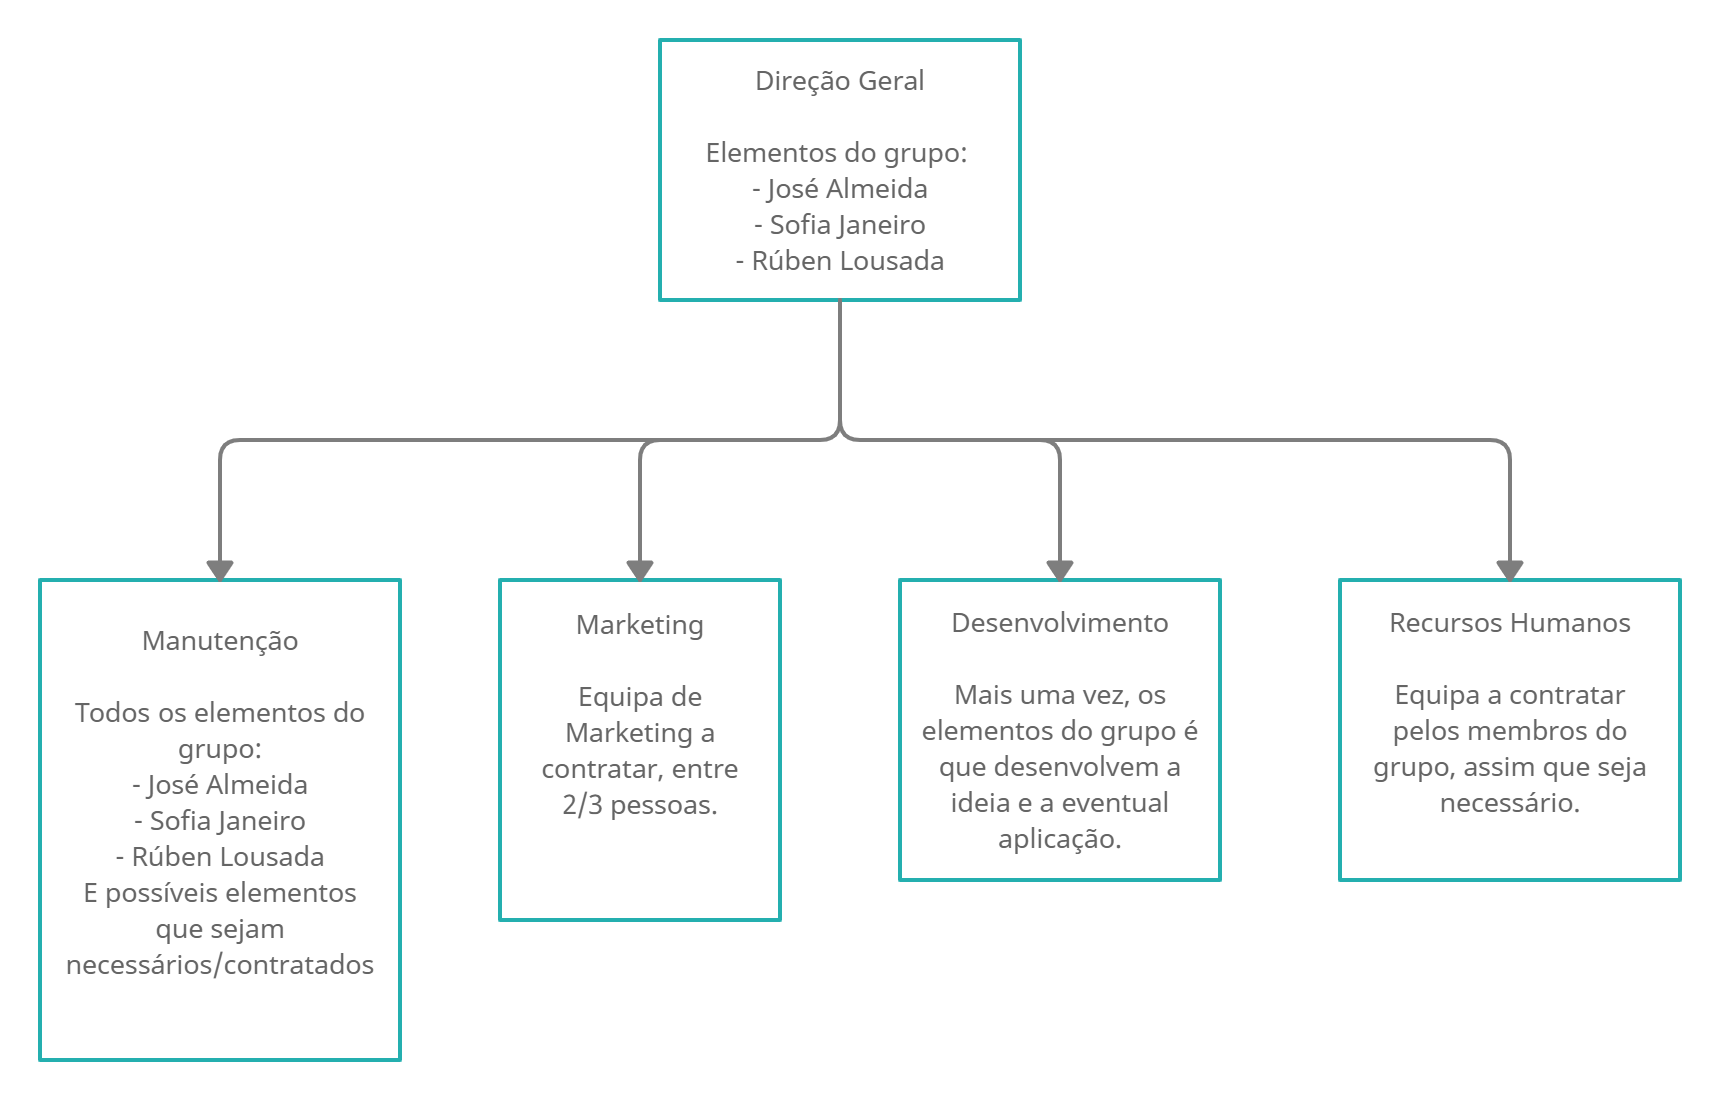
\includegraphics[width=1\textwidth,keepaspectratio]{organigrama}
		\label{fig:organigrama}
		\centering
		\caption{Organigrama}
	\end{figure}
	
	
	\large
	\subsection{Análise da Adequação do Perfil às Funções}
	
	\normalsize
	
	Na fase atual do projeto, ainda não há desenvolvimento suficiente para ser necessário
	pessoal na empresa pelo que consideramos este ponto irrelevante.
	
	
	\large
	\subsection{Processo de Decisão}
	
	\normalsize
	
	As decisões estratégicas da empresa serão tomadas pelos membros do grupo sendo que, futuramente, haverá possivelmente um maior número de pessoas que trabalham em prol da empresa. Os empregados da empresa são maioritariamente autónomos especialmente com a possibilidade de teletrabalho. 
	
	
	\large
	\subsection{Qualificações do Quadro de Recursos Humanos}
	
	\normalsize
	
	No futuro, quando for necessária a contratação de colaboradores para a secção de RH, estes devem ser, no mínimo, licenciados.
	
	
	\large
	\subsection{Gestão de Recursos Humanos}
	
	\normalsize
	
	Inicialmente, os elementos do grupo serão responsáveis pela gestão dos Recursos Humanos e pela atribuição de cada empregado em cada área na empresa. Pretendemos fazer um check-up trimestral sobre os Recursos Humanos. 
	
	
	\large
	\subsection{Profissionais Externos}
	
	\normalsize
	
	Poderão ser necessários profissionais externos, tais como contactos com organizações governamentais como a Conservatória do Registo Predial, Registo Predial Online, Plataforma do Balcão Único
	do Prédio, designada por BUPi. Devem ser criadas parcerias e meios de comunicação com estas organizações.
	
	\pagebreak
	
	\large
	\section{Riscos do Negócio}
	\subsection{Análise Externa - Ameaças e Oportunidades}
	\subsubsection{Ambiente Geral ou Macroambiente}
	
	\footnotesize
	
	\begin{adjustbox}{center}
		\begin{tabular}{|c|l|}
			\hline
			Fatores                                                                               & \multicolumn{1}{c|}{Análise}                                                                                                                                                                                                                                                                                                                                                                                                                                                                                                                                                                                                                                                                                                                                                                                                                                                                                                                                                                                                                                                                                                                                                                                            \\ \hline
			\begin{tabular}[c]{@{}c@{}}Mercado de\\ Trabalho\end{tabular}                         & \begin{tabular}[c]{@{}l@{}}Embora o modelo tradicional de trabalho não vá desaparecer tão depressa, surgem cada vez mais novos\\ modelos, associados à criação de novos produtos e serviços, mais adaptados às transformações sociais \\ inseridas num ritmo de vida mais acelerado, cuja realidade tende a ser cada vez mais digital e que\\ depende/precisa de respostas a necessidades imediatas. Neste contexto, obter uma solução rápida e\\ pouco onerosa, à margem da contratação de serviços de "peritos avaliadores" profissionais cujo serviço\\ prestado importa em encargos muito elevados, é de facto uma mais-valia. É essencial conhecer com \\ detalhe o mercado a explorar, assim como o serviço que se está a comercializar, a concorrência, os \\ preços praticados e adequar as estratégias de modo a que o negócio seja sustentável e lucrativo.\end{tabular}                                                                                                                                                                                                                                                                                                                                      \\ \hline
			Legislação Laboral                                                                    & \begin{tabular}[c]{@{}l@{}}No que diz respeito à legislação laboral, estamos a viver atualmente uma discussão entre centrais\\ sindicais, Governo e partidos quanto à Regulação do emprego nas diversas plataformas para a revisão\\ da lei laboral nacional. Através de um estudo aprofundado redigiu-se o Livro Verde, assente em modelos\\ híbridos de trabalho presencial e à distância numa ótica de equilíbrio na promoção das opotunidades e\\ mitigação dos riscos desta modalidade. \\ Quanto à regulação do trabalho em plataformas digitais, os autores propõem que seja criada "uma\\ presunção de laboralidade para estes trabalhadores" e também "um sistema contributivo e fiscal\\ adaptado a esta nova realidade". "Adequar o sistema de Segurança Social às novas formas de prestar \\ trabalho" é outra das principais linhas de reflexão previstas no Livro Verde.\\ O facto de "o prestador de serviço utilizar isntrumentos de trabalho próprios, bem como o facto de estar\\ dispensado de cumprir deveres de assiduidade e pontualidade e não concorrência, não é incompatível\\ com a existência de uma relação de trabalho dependente entre o prestador e a plataforma digital".\end{tabular} \\ \hline
			\begin{tabular}[c]{@{}c@{}}Sindicatos e grupos\\ de pressão\end{tabular}              & \begin{tabular}[c]{@{}l@{}}Ao nível dos Sindicatos, existe atualmente uma envolvência direta das centrais sindicais, Governo e\\ partidos quanto à Regulação do emprego nas diversas plataformas para a revisão da lei laboral nacional,\\ com base no estudo elaborado via "Livro Verde". Qualquer negócio novo pressupõe a exposição a risco\\ inerentes a grupo de pressão, contudo a adoção de estratégias mais eficientes, e a adaptabilidade\\ constante de legalidade e rigor de trabalho, permitirá à empresa atingir os seus objetivos.\end{tabular}                                                                                                                                                                                                                                                                                                                                                                                                                                                                                                                                                                                                                                                           \\ \hline
			\begin{tabular}[c]{@{}c@{}}Valores e Normas\\ De Vida\end{tabular}                    & \begin{tabular}[c]{@{}l@{}}Na vida, uma boa coexistência depnde de todos nós, sermos capazes de respeitar os direitos e as\\ necessidades dos outros. É necessário termos também a capacidade de entender o comportamento dos\\ indivíduos que são influenciados pelas questões económicas, e que em função disso mudam também os\\ hábitos de compra. Tratam-se de questões sociais que nos dão uma ideia do que as pessoas esperam duma\\ empresa. Por outro lado, existem as questões debatidas ao nível dos meios de comunicação, à nível\\ político e de legalidade que devem determinar a atuação da organização.\end{tabular}                                                                                                                                                                                                                                                                                                                                                                                                                                                                                                                                                                                    \\ \hline
			Políticas sectoriais                                                                  & \begin{tabular}[c]{@{}l@{}}Neste medida, estamos perante uma aplicação que oferece um serviço muito específico destinado a um\\ "público" alvo de clientes, que pretendem garantir o atendimento às suas necessidades objetivas, como\\ por exemplo, proprietários de terrenos, interessados em adquirir ou vender terrenos, etc.\end{tabular}                                                                                                                                                                                                                                                                                                                                                                                                                                                                                                                                                                                                                                                                                                                                                                                                                                                                          \\ \hline
			\begin{tabular}[c]{@{}c@{}}Evolução dos\\ indicadores\\ económicos\end{tabular}       & \begin{tabular}[c]{@{}l@{}}Neste vertente, os indicadores de atividade económica permitem-nos acompanhar a evolução dos principais\\ agregados macroeconómicos, o que em termos mais restritos à empresa, permitem-nos adequar o custo do\\ mesmo consoante a conjuntura se apresente mais ou menos favorável.\end{tabular}                                                                                                                                                                                                                                                                                                                                                                                                                                                                                                                                                                                                                                                                                                                                                                                                                                                                                             \\ \hline
			\begin{tabular}[c]{@{}c@{}}Poder de compra\\ dos consumidores\end{tabular}            & \begin{tabular}[c]{@{}l@{}}Atendendo à especificidade do produto, o qual oferece uma alternativa apetecível à deslocação pessoal ou\\ à contratação de serviços a terceiros, torna-se numa mais-valia. A adequação de custos ou serviços do\\ aplicativo pode ser ajustado perante condições macroeconómicas desfavoráveis.\end{tabular}                                                                                                                                                                                                                                                                                                                                                                                                                                                                                                                                                                                                                                                                                                                                                                                                                                                                                \\ \hline
			\begin{tabular}[c]{@{}c@{}}Distribuição do\\ rendimentos pelas\\ regiões\end{tabular} & \begin{tabular}[c]{@{}l@{}}Este modelo de negócio não é compatível com este quesito, uma vez que, tratando-se de uma plataforma\\ digital, acaba por não implicar uma distribuição desigual por regiões dos respetivos rendimentos.\end{tabular}                                                                                                                                                                                                                                                                                                                                                                                                                                                                                                                                                                                                                                                                                                                                                                                                                                                                                                                                                                        \\ \hline
			\begin{tabular}[c]{@{}c@{}}Processos e\\ métodos produtivos\end{tabular}              & \begin{tabular}[c]{@{}l@{}}É de todo interesse que haja uma boa coexistência entre as pessoas responsáveis pela gestão do negócio.\\ Essa base de sustentação permite depois alicerçar os restantes processos que são necessários para obter\\ resultados positivos, nomeadamente no que diz respeito à distribuição de tarefas, internas ou externas,\\ definição equitativa de horários, adequar as ferramentas de trabalho às necessidades existentes por forma\\ a otimizar ao máximo as tarefas para que elas sejam realizadas em menos tempo. Por último, e não menos\\ importante, manter um alinha aberta com os clientes, por forma a gerir as "criticas", reclamações, e dar\\ resposta às mesmas em tempo útil, procurando explicar o funcionamento do produto, sempre que solicitado,\\ ou tentar eliminar/melhorar "bugs" sempre que detetados.\end{tabular}                                                                                                                                                                                                                                                                                                                                               \\ \hline
		\end{tabular}
	\end{adjustbox}


	\begin{adjustbox}{center}
		\begin{tabular}{|c|l|}
			\hline
			Fatores                                                                         & \multicolumn{1}{c|}{Análise}                                                                                                                                                                                                                                                                                                                                                                                                                                                                                                                                                                                                                                                                                                                                                                                                                                                                                                                                                                                                                                                                                                                                                                                    \\ \hline
			Novas tecnologias                                                               & \begin{tabular}[c]{@{}l@{}}As novas tecnologias são algo inevitável num mundo em que grandes tranformações de processos físicos e\\ digitais está em curso. Novas tecnologias estão a ser criadas e desenvolvidas a cada dia que passa e todos\\ sabemos que revoluções deste tipo têm o poder de mudar os negócios. Ouvimos falar constantemente em\\ "realidade virtual", "big data", "trabalho remoto", "computação em nuvem", "mobilidade", "acessibilidade"\\ e "visibilidade", etc.\\ É imprescindível que as empresas se atualizem para atender às novas exigências tecnológicas do mundo. O\\ processo de inovar inicia-se com propósito de criar uma vantagem estratégica no mercado. Por esse motivo,\\ desenvolver um pensamento estratégico é essencial.\\ Isso significa que nessa fase é necessário pensar especificamente sobre como a inovação vai influenciar nos\\ objetivos estratégicos da empresa. Aqui, é necessário estudar as áreas-alvo em que a inovação tem mais\\ hipóteses de fornecer uma vantagem estratégica.\\ Depois de observar as necessidades e a evolução do mercado, há que listar as opções que podem ajudar a\\ continuar a fazer a diferença no negócio.\end{tabular} \\ \hline
			\begin{tabular}[c]{@{}c@{}}Politica de\\ Investigação\\ Cientifica\end{tabular} & \begin{tabular}[c]{@{}l@{}}O primeiro passo é determinado pela criação da aplicação, estudo da sua aplicabilidade e potenciais ramificações, \\ para depois passar a uma fase de testes.  Os testes devem, numa primeira abordagem, possibilitar a comprovação \\ de que os resultados obtidos no formato digital, correspondam a uma medição real no respetivo local, por forma a \\ observar que a leitura obtida é de facto a correta, admitindo-se que haja sempre uma pequena margem de erro. \\ Como em qualquer estudo científico, importa colocar questões sobre a utilização dessa ferramenta e testar múltiplas \\ vezes o seu funcionamento e respetivos resultados por forma a comprovar que os mesmos são fidedignos, e para \\ que isso aconteça, é necessário realizar testes precisos.\end{tabular}                                                                                                                                                                                                                                                                                                                                                                                             \\ \hline
		\end{tabular}
	\end{adjustbox}
	
	
	\large
	\subsubsection{Ambiente da Indústria ou Competitivo}
	
	\normalsize
	
	\begin{adjustbox}{center}
		\begin{tabular}{|c|c|}
			\hline
			Fatores      & Análise                                                                                                                                                                                                                                                                                                                                                                           \\ \hline
			Clientes     & \begin{tabular}[c]{@{}c@{}}Inicialmente teremos um poder negocial alto visto que haverá\\ pouca procura em relação à quantidade de fornecedores mas, com\\ o passar do tempo temos boas expectativas para que este venha a\\ diminuir.\end{tabular}                                                                                                                               \\ \hline
			Concorrentes & \begin{tabular}[c]{@{}c@{}}Consideramos que a rivalidade entre nós e os nossos concorrentes é \\ saudável visto que respeitamos todos os 'players' neste mercado de\\ trabalho. É importanto referir que, com a esperança de um futuro\\ próspero para a empresa, a rivalidade venha a aumentar mas esperemos\\ e faremos com que a ideia inicial permaneça intacta.\end{tabular} \\ \hline
			Sector       & \begin{tabular}[c]{@{}c@{}}Visto que não há um número elevado de concorrência, é seguro afirmar\\ que este setor não está saturado. Dito isto, o processo de expansão é \\ facilitado, podendo assim explorar features que não existem no mercado\\ ou mesmo melhorar/expandir as ideias que já existem.\end{tabular}                                                             \\ \hline
		\end{tabular}
	\end{adjustbox}
	
	\large
	\subsubsection{Análise Interno - Forças e Fraquezas}
	
	\normalsize
	
	\begin{adjustbox}{center}
		\begin{tabular}{|c|c|}
			\hline
			Fatores                                                            & Análise                                                                                                                                                                                                                                                                                                            \\ \hline
			Situação histórica                                                 & \begin{tabular}[c]{@{}c@{}}Estamos a levar o nosso tempo para desenvolver a ideia mas acreditamos\\ que a evolução vai ser favorável e que vai valer a pena o esforço e dedicação\\ posta por todos os membros do grupo.\end{tabular}                                                                              \\ \hline
			Situação económica                                                 & \begin{tabular}[c]{@{}c@{}}Devido a um estudo de mercado feito anteriormente, sabemos que existem\\ bastantes clientes interessados e que temos um futuro promissor com a nossa\\ ideia. Quanto à viabilidade financeira, sabemos que precisamos de ajuda porém\\ não vemos isso como um impedimento.\end{tabular} \\ \hline
			Situação financeira                                                &                                                                                                                                                                                                                                                                                                                    \\ \hline
			\begin{tabular}[c]{@{}c@{}}Sistema de\\ Informática\end{tabular}   & \begin{tabular}[c]{@{}c@{}}Visto que somos todos alunos de Engenharia Informática, podemos afirmar que\\ a circulação de informação entre nós é feita de forma eficiente.\end{tabular}                                                                                                                             \\ \hline
			\begin{tabular}[c]{@{}c@{}}Estrutura\\ organizacional\end{tabular} &                                                                                                                                                                                                                                                                                                                    \\ \hline
		\end{tabular}
	\end{adjustbox}
	
	
	\large
	\subsection{Análise SWOT}
	
	\scriptsize

	\begin{adjustbox}{center}
		\begin{tabular}{|c|c|c|c|}
			\hline
			\multicolumn{2}{|c|}{\multirow{2}{*}{}}                                                                                                                                              & Ameaças                                                                                                                                                                                                           & Oportunidades                                                                                                                                                                                                                                                 \\ \cline{3-4} 
			\multicolumn{2}{|c|}{}                                                                                                                                                               & \begin{tabular}[c]{@{}c@{}}Somos uma empresa nova \\ no mercado, com pouco \\ poder financeiro. Mesmo que tenhamos\\ inovação do nosso lado, os nossos concorrentes\\  têm mais poder e experiência.\end{tabular} & \begin{tabular}[c]{@{}c@{}}Com o desenvolvimento desta ideia\\ e com ajuda financeira por parte de\\ investidores, teremos oportunidade\\  de lançar uma nova ideia para o mercado \\ que será, possivelmente vantajosa para\\  ambas as partes.\end{tabular} \\ \hline
			Forças    & \begin{tabular}[c]{@{}c@{}}A nossa app tem features únicas, \\ que os nossos concorrentes\\ não possuem, daí ser uma inovação.\end{tabular}                              & \begin{tabular}[c]{@{}c@{}}Desenvolvimento da ideia e da aplicação porém,\\ pouca aderência por parte dos clientes.\end{tabular}                                                                                  & \begin{tabular}[c]{@{}c@{}}Sucesso da empresa, desenvolvimento da\\ aplicação e colocação da mesma no mercado\\  de trabalho. Contratação de uma equipa que\\ venha a gerir a empresa com o grupo inicial.\end{tabular}                                       \\ \hline
			Fraquezas & \begin{tabular}[c]{@{}c@{}}As gerações atuais não compram/cuidam \\ de terrenos como as gerações anteriores\\ pelo que a afluência deste mercado\\ é menor.\end{tabular} & Fracasso da empresa.                                                                                                                                                                                              & \begin{tabular}[c]{@{}c@{}}Desenvolvimento da ideia e da aplicação \\ porém, pouca aderência\\ por parte dos clientes.\end{tabular}                                                                                                                           \\ \hline
		\end{tabular}
	\end{adjustbox}
	
	
	\large
	\subsection{Modelo das 5 Forças de Porter}
	\subsubsection{Ameaça de Novas Entradas}
	
	\normalsize
	
	\begin{adjustbox}{center}
		\begin{tabular}{|l|l|}
			\hline
			Factores                                                                                                                                                                                                 & S/N?                                                                                                                                       \\ \hline
			1. As economias de escalas são baixas?                                                                                                                                                                   & S                                                                                                                                          \\ \hline
			2. A diferenciação é baixa?                                                                                                                                                                              & S                                                                                                                                          \\ \hline
			3. As necessidades de capital não são elevadas?                                                                                                                                                          & N                                                                                                                                          \\ \hline
			4. Os custos que incorrem da mudanças de fornecedor são reduzidos?                                                                                                                                       & N                                                                                                                                          \\ \hline
			5. Os canais de distribuição são de fácil acesso?                                                                                                                                                        & S                                                                                                                                          \\ \hline
			6. Não existem políticas governamentais restritivas?                                                                                                                                                     & S                                                                                                                                          \\ \hline
			7. A tecnologia necessária é acessível?                                                                                                                                                                  & S                                                                                                                                          \\ \hline
			\multicolumn{2}{|l|}{Análise}                                                                                                                                                                                                                                                                                                                         \\ \hline
			\multicolumn{2}{|l|}{\begin{tabular}[c]{@{}l@{}}O mercado de trabalho é uma indústria em constante crescimento. Tendo isso em conta, achamos que a nossa ideia\\ de negócio é atrativa e necessária visando os nossos concorrentes, pois temos pontos suficientemente\\ fortes e inovadores para garantir uma fácil entrada no mercado.\end{tabular}} \\ \hline
		\end{tabular}
	\end{adjustbox}
	
	\large
	\subsubsection{Ameaça de Serviços Substitutos}
	
	\normalsize
	
	\begin{adjustbox}{center}
		\begin{tabular}{|c|c|}
			\hline
			Factores                                                                                                                                                                 & S/N?                                                           \\ \hline
			\multicolumn{1}{|l|}{1. A rentabilidade económica obtida com a prestação de um serviço substituto é superior?}                                                           & S                                                              \\ \hline
			\multicolumn{1}{|l|}{2. Relação preço/desempenho do produto/serviço susbtituto é superior?}                                                                              & N                                                              \\ \hline
			\multicolumn{2}{|c|}{Análise}                                                                                                                                                                                                             \\ \hline
			\multicolumn{2}{|c|}{\begin{tabular}[c]{@{}c@{}}Consideramos que a nossa ideia seja muito inovadora devido à quantidade de features diferentes\\ temos, daí não sentirmos ameaça de possíveis substitutos do nosso serviço.\end{tabular}} \\ \hline
		\end{tabular}
	\end{adjustbox}
	
	
	\large
	\subsubsection{Rivalidade Entre os Concorrentes}
	
	\normalsize
	
	\begin{adjustbox}{center}
		\begin{tabular}{|l|c|}
			\hline
			\multicolumn{1}{|c|}{Factores}                                                                                                                                                                & S/N?                         \\ \hline
			1. O número de concorrentes é elevado?                                                                                                                                                        & N                            \\ \hline
			2. Os custos fixos ou de armazenagem são elevados?                                                                                                                                            & N                            \\ \hline
			3. A diferenciação do produto é baixa?                                                                                                                                                        & S                            \\ \hline
			\begin{tabular}[c]{@{}l@{}}4. As empresas estão dispostas a sacrificar a rentabilidade de curto prazo, em função do\\ interesse estratégico do negócio?\end{tabular}                          & N                            \\ \hline
			\multicolumn{2}{|c|}{Análise}                                                                                                                                                                                                \\ \hline
			\multicolumn{2}{|l|}{\begin{tabular}[c]{@{}l@{}}A nossa app dispõe de serviços únicos visto que não são oferecidos pelos nossos concorrentes por\\ isso estamos seguros que trazemos algo inovador ao mercado.\end{tabular}} \\ \hline
		\end{tabular}
	\end{adjustbox}
	
	
	\large
	\subsubsection{Poder Negocial dos Clientes}
	
	\normalsize
	
	\begin{adjustbox}{center}
		\begin{tabular}{|l|c|}
			\hline
			\multicolumn{1}{|c|}{Factores}                                                                                                                                     & S/N?                                                                                                 \\ \hline
			1. Existe concentração elevada de cliente?                                                                                                                         & N                                                                                                    \\ \hline
			2. As compras dos clientes têm grande impacto na empresa?                                                                                                          & N                                                                                                    \\ \hline
			3. Os produtos/serviços são pouco diferenciáveis?                                                                                                                  & S                                                                                                    \\ \hline
			4. O produto/serviço possui um peso elevado nos custos do cliente?                                                                                                 & N                                                                                                    \\ \hline
			\multicolumn{2}{|c|}{Análise}                                                                                                                                                                                                                                             \\ \hline
			\multicolumn{2}{|c|}{\begin{tabular}[c]{@{}c@{}}Inicialmente teremos um poder negocial alto visto que haverá pouca procura \\ em relação à quantidade de fornecedores mas, com o passar do tempo temos \\ boas expectativas para que este venha a diminuir.\end{tabular}} \\ \hline
		\end{tabular}
	\end{adjustbox}
	
	
	\large
	\subsubsection{Poder Negocial dos Fornecedores}
	
	\normalsize
	
	\begin{adjustbox}{center}
		\begin{tabular}{|l|c|}
			\hline
			\multicolumn{1}{|c|}{Factores}                                                                                                                        & S/N?                                                                \\ \hline
			1. Existe uma concentração elevada de fornecedores de um determinado produto/serviço?                                                                 & N                                                                   \\ \hline
			2. Inexistência de produtos/serviços substitutos?                                                                                                     & N                                                                   \\ \hline
			3. A diferenciação dos produtos/serviços dos fornecedores é elevada?                                                                                  & N                                                                   \\ \hline
			4. A indústria a abastecer não constitui um cliente importante?                                                                                       & N                                                                   \\ \hline
			5. A importância do produto/serviço para o comprador é elevada?                                                                                       & S                                                                   \\ \hline
			\multicolumn{2}{|c|}{Análise}                                                                                                                                                                                               \\ \hline
			\multicolumn{2}{|l|}{\begin{tabular}[c]{@{}l@{}}Atendendo ao facto de que pretendemos disponibilizar produtos e serviços através do meio digital,\\ os fornecedores não serão, à partida, relevantes.\end{tabular}} \\ \hline
		\end{tabular}
	\end{adjustbox}
	
	\pagebreak
	
	\large
	\section{Plano de Implementação}
	
	\normalsize

	Existem 6 etapas que consideramos ser principais na criação, crescimento e manutenção da nossa empresa. São as seguintes:
	
	\large
	\subsection{Etapa 1 - Protótipo}
	\normalsize
	
	Inicialmente, será desenvolvido um protótipo, com funcionalidades básicas essenciais à aplicação. Deve ser recolhida o máximo de informação sobre a user experience desse protótipo, que será tomada em conta na etapa seguinte. Os recursos necessários a esta etapa são baixos, pois o desenvolvimento é realizado pela nossa equipa, sem remuneração. Estimamos que esta etapa dure cerca de 3 meses.
	
	\large
	\subsection{Etapa 2 - Refinar e implementar funcionalidades}
	\normalsize
	
	Com o user feedback recebido, a aplicação será refinada de modo a se adaptar ao máximo às necessidades e dificuldades sentidas pelos seus clientes. Seguidamente, serão implementadas mais funcionalidades, sempre tendo em conta o user feedback recebido. Como na etapa 1, os recursos necessários são baixos, embora possivelmente incluam custos como licenças de uso de software, entre outros. Estimamos que esta etapa dure cerca de 9 meses.
	
	\large
	\subsection{Etapa 3 - Introdução no mercado nacional}
	\normalsize
	
	Com a aplicação finalmente desenvolvida, esta será lançada nos mercados de aplicações como o Google Play e App Store. No entanto, estará ainda restrita a Portugal. Esta etapa terá mais custos associados que as anteriores, pois é necessária infraestrutura (servidores, escritório, ...), assim como uma equipa. Estimamos que esta etapa dure cerca de 1 ano.
	
	\large
	\subsection{Etapa 4 - Manter, refinar e implementar funcionalidades}
	\normalsize
	
	Durante o ano seguinte à introdução no mercado nacional, a aplicação será mantida, refinada e alterada, com o objetivo de a preparar para a internacionalização do ano seguinte. Os custos desta etapa passarão por um aumento da equipa, assim como nos equipamentos associados. Estimamos que esta etapa dure cerca de 1 ano.
	
	\large
	\subsection{Etapa 5 - Introdução no mercado internacional}
	\normalsize
	
	Estando a aplicação estabilizada no mercado nacional, esta será, então, aberta para o mercado internacional, procurando atingir o maior número de pessoas do nosso público-alvo. Com isto, terá de haver um claro crescimento rápido não só da equipa, como de todos os custos, em geral, fazendo esta etapa a mais dispendiosa, em termos de investimento inicial. Estimamos que esta etapa dure cerca de 3 anos.
	
	\pagebreak
	
	\large
	\subsection{Etapa 6 - Manutenção, crescimento e implementação periódica de funcionalidades}
	\normalsize
	
	Com a aplicação introduzida em todo o mundo, o objetivo principal passa por manter a mesma, continuando a investir de modo a garantir o seu sucesso ao longo do tempo. Serão, também, introduzidas periodicamente novas funcionalidades, que se revelarem pertinentes. Esta etapa não tem duração estimada.
	
	\large
	\subsection{Bootstrapping}
	\normalsize
	
	No caso de, em qualquer uma das etapas, nos encontrarmos sem os fundos esperados para realizar o plano inicial, iremos recorrer a medidas como:
	
	\begin{itemize}
		\item Diminuir os gastos com o escritório, incentivando o tele-trabalho;
		\item Extender o prazo das etapas;
		\item Reduzir o número de colaboradores para o essencial.
	\end{itemize}
	
	\pagebreak
	
	\large
	\section{Análise da Viabilidade Económica e Financeira}
	\subsection{Investimento e Financiamento Previsionais}
	
	\normalsize
	
	Cada ano, com a entrada de novos colaboradores para a equipa, será obrigatória a compra de novos materiais para os mesmos. Têm de ser igualmente adquiridos computadores de trabalho para cada novo elemento. O número de bens na tabela equivale ao número de colaboradores a ser contratados todos os anos.
	
	\small
	\begin{adjustbox}{center}
		\begin{tabular}{|l|l|l|l|l|l|}
			\multicolumn{1}{l}{} & \multicolumn{1}{l}{} & \multicolumn{1}{l}{} & \multicolumn{1}{l}{Valores s/ IVA} & \multicolumn{1}{l}{} & \multicolumn{1}{l}{Euros} \\ \hline
			NR. ORDEM                 & RÚB. INVESTIMENTO & DATA AQUISIÇÃO & QUANTIDADE & VALOR unidade & VALOR total \\ \hline
			1                         &        Computadores      &    2021        &       0     &      900      &      0       \\ \hline
			2                         &        Mobiliário        &      2021      &     0       &   400         &     0        \\ \hline
			3                         &        Computadores      &    2022        &       1     &      900      &      900       \\ \hline
			4                         &        Mobiliário        &      2022      &     1       &   400         &     400        \\ \hline
			5                         &        Computadores      &    2023        &       4     &      900      &      3600       \\ \hline
			6                         &        Mobiliário        &      2023      &     4       &   400         &     1600        \\ \hline
			7                         &        Computadores      &    2024        &       8     &      900      &      7200       \\ \hline
			8                         &        Mobiliário        &      2024      &     8       &   400         &     3200        \\ \hline
			\multicolumn{5}{r}{TOTAL Investimento} & \multicolumn{1}{r}{16,800} \\ 
		\end{tabular}
	\end{adjustbox}
	\normalsize
	
	\begin{center}
		\begin{tabular}{|l|l|r|r|r|r|r|}
			\hline
			\multicolumn{1}{|c|}{Investimento por ano}           & 2021 & \multicolumn{1}{l|}{2022} & \multicolumn{1}{l|}{2023} & \multicolumn{1}{l|}{2024} & \multicolumn{1}{l|}{2025} & \multicolumn{1}{l|}{2026} \\ \hline
			ATIVOS FIXOS TANGÍVEIS                               &      &                           &                           &                           &                           &                           \\ \hline
			Equipamento Básico                                   &      & 15,000                    & 15,000                    & 50,000                    & 55,000                    & 62,000                    \\ \hline
			Equipamento de Transporte                            &      &                           &                           &                           &                           &                           \\ \hline
			Terrenos e recursos naturais                         &      &                           &                           &                           &                           &                           \\ \hline
			Edifícios e outras Construções                       &      &                           &                           &                           &                           &                           \\ \hline
			Total Ativos Fixos Tangíveis                         &      & 15,000                    & 15,000                    & 50,000                    & 55,000                    & 62,000                    \\ \hline
			\multicolumn{1}{l}{} & \multicolumn{1}{l}{} & \multicolumn{1}{l}{} & \multicolumn{1}{l}{} & \multicolumn{1}{l}{} & \multicolumn{1}{l}{} & \multicolumn{1}{l}{} \\ \hline
			ATIVOS FIXOS INTANGÍVEIS                             &      &                           &                           &                           &                           &                           \\ \hline
			Projetos de desenvolvimento                          &      & 1,500                     & 1,000                     & 1,600                     & 1,600                     & 1,600                     \\ \hline
			Software                                             &      &                           &                           &                           &                           &                           \\ \hline
			Propriedade industrial                               &      &                           &                           &                           &                           &                           \\ \hline
			Goodwill                                             &      &                           &                           &                           &                           &                           \\ \hline
			\multicolumn{1}{|c|}{Total Ativos Fixos Intangíveis} &      & 1,500                     & 1,000                     & 1,600                     & 1,600                     & 1,600                     \\ \hline
			Total Investimento                                   &      & 16,500                    & 16,000                    & 51,600                    & 56,600                    & 63,300                    \\ \hline
		\multicolumn{1}{l}{} & \multicolumn{1}{l}{} & \multicolumn{1}{l}{} & \multicolumn{1}{l}{} & \multicolumn{1}{l}{} & \multicolumn{1}{l}{} & \multicolumn{1}{l}{} \\ \hline
			FINANCIAMENTO DO INVESTIMENTO          & 2021 & 2022 & 2023 & 2024 & 2025 & 2026 \\ \hline
			CAPITAIS PRÓPRIOS                      & 3,000 & 0    & 0    & 0 & &   \\ \hline 
			Capital Social                         & 3,000 & 0    & 0    & 0  & & \\ \hline
			Prestações suplementares               & 0    & 0    & 0    & 0  & &  \\ \hline
			AUTOFINANCIAMENTO                      &      &      &      &   & &  \\ \hline
			CAPITAIS ALHEIOS                       &      &      &      &   & &  \\ \hline
			Empréstimos bancários                  &      &50,000& 220,000&   & &  \\ \hline
			Empréstimos de sócios (Suprimentos)    &      &      &       &    & &   \\ \hline
			Crédito de fornecedores de Imobilizado &      &      &      &    & &   \\ \hline
			Outros                                 &      &      &      &    & &   \\ \hline
			TOTAL (c/ autofinanciamento)           & 5,000 & 50,000     & 220,000    & &  & \\ \hline
		\end{tabular}
	\end{center}

	\pagebreak
	
	\large
	\subsection{Proveitos e Custos Previsionais}
	
	\normalsize
	
	\begin{adjustbox}{center}
		\begin{tabular}{|l|r|r|r|r|r|}
			\multicolumn{1}{l}{VENDAS - MERCADO NACIONAL} & \multicolumn{1}{c}{2021} & \multicolumn{1}{c}{2022} & \multicolumn{1}{c}{2023} & \multicolumn{1}{c}{2024} & \multicolumn{1}{c}{2025} \\ \hline
			PLANO LIFETIME - NÚMERO ILIMITADO DE TERRENOS  & - & 4,485                    & 7,176                  & 9,688                   & 12,594                   \\ \hline
			Quantidades vendidas                           &                -          & 1,500                    & 2,400                    & 3,240                    & 4,212                    \\ \hline
			Taxa de crescimento das unidades vendidas      &           -               & -                  & 60.00\%                  & 35.00\%                  & 30.00\%                  \\ \hline
			Preço Unitário                                 &         -                 & 2.99                     & 2.99                     & 2.99                     & 2.99                     \\ \hline
			\multicolumn{1}{r}{TOTAL:} & \multicolumn{1}{r}{0} & \multicolumn{1}{r}{4,485} & \multicolumn{1}{r}{7,176} & \multicolumn{1}{r}{9,688} & \multicolumn{1}{r}{12,594} \\
			\multicolumn{1}{l}{} & \multicolumn{1}{l}{} & \multicolumn{1}{l}{} & \multicolumn{1}{l}{} & \multicolumn{1}{l}{} & \multicolumn{1}{l}{} \\
			\multicolumn{1}{l}{PRESTAÇÕES DE SERVIÇOS - MERCADO NACIONAL} & \multicolumn{1}{l}{}& \multicolumn{1}{l}{} & \multicolumn{1}{l}{} & \multicolumn{1}{l}{} & \multicolumn{1}{l}{}\\ \hline
			SUBSCRIÇÃO MENSAL - ANUNCIOS NO MERCADO        &     -                     & 6,000                    & 9,600                   & 12,960                   & 17,496                   \\ \hline
			Taxa de crescimento                            &         -                 &               -           & 60.00\%                  & 35.00\%                  & 35.00\%                  \\ \hline
			SUBSCRIÇÃO MENSAL - Cultivos                   &         -                 & 3,000                    & 4,800                    & 6,480                   & 8,748                   \\ \hline
			Taxa de crescimento                            &                  -        &          -                & 60.00\%                  & 35.00\%                  & 35.00\%                  \\ \hline
			SUBSCRIÇÃO MENSAL - Premium                    &              -            & 1,500                     & 2,400                    & 3,240                    & 4,374                    \\ \hline
			Taxa de crescimento                            &               -           &         -                 & 60.00\%                  & 35.00\%                  & 35.00\%                  \\ \hline
			\multicolumn{1}{r}{TOTAL:} & \multicolumn{1}{r}{0} & \multicolumn{1}{r}{10,500} & \multicolumn{1}{r}{16,800} & \multicolumn{1}{r}{22,680} & \multicolumn{1}{r}{30,618} \\
			\multicolumn{1}{l}{} & \multicolumn{1}{l}{} & \multicolumn{1}{l}{} & \multicolumn{1}{l}{} & \multicolumn{1}{l}{} & \multicolumn{1}{l}{} \\
			\multicolumn{1}{l}{VENDAS - MERCADO INTERNACIONAL} & \multicolumn{1}{l}{}& \multicolumn{1}{l}{} & \multicolumn{1}{l}{} & \multicolumn{1}{l}{} & \multicolumn{1}{l}{}\\ \hline
			PLANO LIFETIME - NÚMERO ILIMITADO DE TERRENOS  & -                        & -                   & -                       &  104,650                       & 261,625                         \\ \hline
			Quantidades vendidas                           &        -                  & -                        & -                      & 35,000                       &         87,500                 \\ \hline
			Taxa de crescimento das unidades vendidas      &     -                     & -                   & - & -  & 150.00\%                               \\ \hline
			Preço unitario                                 &              -            & -                     & -                     & 2.99                     &           2.99               \\ \hline
			\multicolumn{1}{r}{TOTAL:} & \multicolumn{1}{r}{0} & \multicolumn{1}{r}{0} & \multicolumn{1}{r}{0} & \multicolumn{1}{r}{104,650} & \multicolumn{1}{r}{261,625} \\
			\multicolumn{1}{l}{} & \multicolumn{1}{l}{} & \multicolumn{1}{l}{} & \multicolumn{1}{l}{} & \multicolumn{1}{l}{} & \multicolumn{1}{l}{} \\
			\multicolumn{1}{l}{PRESTAÇÕES DE SERVIÇOS - MERCADO INTERNACIONAL} & \multicolumn{1}{l}{}& \multicolumn{1}{l}{} & \multicolumn{1}{l}{} & \multicolumn{1}{l}{} & \multicolumn{1}{l}{}\\ \hline
			SUBSCRIÇÃO MENSAL - ANÚNCIOS NO MERCADO        & -                   & -                  & -                & 400,000                &               1,000,000           \\ \hline
			Taxa de crescimento                            &              -            &            -              & -                 & -                  &      150.00\%                    \\ \hline
			SUBSCRIÇÃO MENSAL - Cultivos                   & -                        & -                  & -                  & 170,000                 &        425,000                  \\ \hline
			Taxa de crescimento                            &            -              &                -          & -                & -                 &     150.00\%                     \\ \hline
			SUBSCRIÇÃO MENSAL - Premium                    & -                        & -                 & -                  & 300,000               &      750,000                    \\ \hline
			Taxa de crescimento                            &                   -       &               -           & -                & -                 &  15.00\%                        \\ \hline
			\multicolumn{1}{r}{TOTAL:} & \multicolumn{1}{r}{0} & \multicolumn{1}{r}{0} & \multicolumn{1}{r}{0} & \multicolumn{1}{r}{870,000} & \multicolumn{1}{r}{2,175,000}                   
		\end{tabular}
	\end{adjustbox}

	\vspace{1cm}

	Acreditamos que, nos primeiros meses da vida da aplicação, a sua popularidade não seja muito elevada, sendo preciso publicitá-la. Durante o desenvolvimento da aplicação, está não será promovida. Após um ano da sua publicação, será promovida tendo como objetivo aumentar em 60\% o número dos clientes, chegando, assim, ao seu ápice de aumento de clientes nacionais. Ao longo dos próximos anos, o aumento de clientes nacionais irá decrescer. Em 2024, ano da expansão internacional, é previsto um crescimento de cerca de 400 mil clientes, obtendo, no ano seguinte, um aumento de 150\% de utilizadores.

	\tiny
	\begin{adjustbox}{center}
		\begin{tabular}{|l|l|l|l|l|l|l|l|l|l|l|}
			\hline
			& Taxa IVA & CF      & CV     & Valor Mensal & 2021 & 2022      & 2023      & 2024       & 2025       & 2026       \\ \hline
			Subcontratos                                & 23.0\%   & 100.0\% &        &              &      &           &           &            &            &            \\ \hline
			SERVIÇOS ESPECIALIZADOS                    &          &         &        &              &      &           &           &            &            &            \\ \hline
			Trabalhos especializados                    & 23.0\%   & 100.0\% &        &              &      &           &           &            &            &            \\ \hline
			Publicidade e propaganda                    & 23.0\%   & 50.0\%  & 50.0\% & 500.00       &      & 5,000.00  & 6,900.00  & 34,500.00  & 39,675.00  & 47,610.00  \\ \hline
			Vigilância e segurança                      & 23.0\%   & 100.0\% &        &              &      &           &           &            &            &            \\ \hline
			Honorários                                  & 23.0\%   & 100.0\% &        &              &      &           &           &            &            &            \\ \hline
			Comissões                                   & 23.0\%   & 100.0\% &        &              &      &           &           &            &            &            \\ \hline
			Conservação e reparação                     & 23.0\%   & 100.0\% &        &              &      &           &           &            &            &            \\ \hline
			MATERIAIS                                   &          &         &        &              &      &           &           &            &            &            \\ \hline
			Ferramentas e utensilios de desgaste rápido & 23.0\%   & 100.0\% &        &              &      &           &           &            &            &            \\ \hline
			Livros e documentação técnica               & 23.0\%   & 100.0\% &        &              &      &           &           &            &            &            \\ \hline
			Material de escritório                      & 23.0\%   & 50.0\%  & 50.0\% & 100.00       &      & 1,000.00  & 1,380.00  & 6,900.00   & 7, 935.00  & 9,522.00   \\ \hline
			Artigos para oferta                         & 23.0\%   & 100.0\% &        &              &      &           &           &            &            &            \\ \hline
			ENERGIA E FLUIDOS                           &          &         &        &              &      &           &           &            &            &            \\ \hline
			Eletricidade                                & 23.0\%   & 80.0\%  & 20.0\% & 100.00       &      & 1,000.00  & 1380.00   & 6,900.00   & 7, 935.00  & 9,522.00   \\ \hline
			Combustíveis                                & 23.0\%   & 100.0\% &        &              &      &           &           &            &            &            \\ \hline
			Água                                        & 6.0\%    & 80.0\%  & 20.0\% & 20.00        &      & 200.00    & 276.00    & 1380.00    & 1587.00    & 1904.40    \\ \hline
			DESLOCAÇÕES, ESTADIAS E TRANSPORTES          &          &         &        &              &      &           &           &            &            &            \\ \hline
			Deslocações e Estadias                       & 23.0\%   & 100.0\% &        &              &      &           &           &            &            &            \\ \hline
			Transportes de pessoal                      & 23.0\%   & 100.0\% &        &              &      &           &           &            &            &            \\ \hline
			Transportes de mercadorias                  & 23.0\%   & 100.0\% &        &              &      &           &           &            &            &            \\ \hline
			SERVIÇOS DIVERSOS                          &          &         &        &              &      &           &           &            &            &            \\ \hline
			Rendas e alugueres                          & 23.0\%   & 100.0\% &        & 2,000.00     &      & 20,000.00 & 27,600.00 & 138,000.00 & 158,700.00 & 194,440.00 \\ \hline
			Comunicação                                 & 23.0\%   & 100.0\% &        & 100.00       &      & 1,000.00  & 1380.00   & 6,900.00   & 7,935.00   & 9,522.00   \\ \hline
			Seguros                                     &          & 100.0\% &        &              &      &           &           &            &            &            \\ \hline
			Royalties                                   & 23.0\%   & 100.0\% &        &              &      &           &           &            &            &            \\ \hline
			Contencioso e notariado                     & 23.0\%   & 100.0\% &        &              &      &           &           &            &            &            \\ \hline
			Despesas de representação                   & 23.0\%   & 100.0\% &        &              &      &           &           &            &            &            \\ \hline
			Limpeza, higiene e conforto                 & 23.0\%   & 100.0\% &        &              &      &           &           &            &            &            \\ \hline
			OUTROS SERVIÇOS                             & 23.0\%   & 100.0\% &        &              &      &           &           &            &            &            \\ \hline
			\multicolumn{6}{|c|}{TOTAL FSE}                                                                 & 28,200.00 & 38,916.00 & 194,580.00 & 223,767.00 & 268,520.40 \\ \hline
			&          &         &        &              &      &           &           &            &            &            \\ \hline
			\multicolumn{5}{|l|}{FSE - Custos Fixos}                                                 &      & 24,960.00 & 34,444.80 & 172,224.00 & 198,057.60 & 237,669.12 \\ \hline
			&          &         &        &              &      &           &           &            &            &            \\ \hline
			\multicolumn{5}{|l|}{FSE - Custos Variáveis}                                             &      & 3,240.00  & 4,471.00  & 22,356.00  & 25,709.40  & 30,851.00  \\ \hline
			&          &         &        &              &      &           &           &            &            &            \\ \hline
			\multicolumn{5}{|l|}{TOTAL FSE}                                                          &      & 28,200.00 & 38,916.00 & 194,580.00 & 223,767.00 & 268,520.40 \\ \hline
			&          &         &        &              &      &           &           &            &            &            \\ \hline
			\multicolumn{5}{|l|}{IVA}                                                                &      & 1,852.00  & 2,555.76  & 12,778.00  & 14,695.00  & 17,634.74  \\ \hline
			&          &         &        &              &      &           &           &            &            &            \\ \hline
			\multicolumn{5}{|l|}{FSE + IVA}                                                          &      & 30,052.00 & 41,471.76 & 207,358.00 & 238,462.62 & 286,155.14 \\ \hline
		\end{tabular}
	\end{adjustbox}

	\normalsize
	\begin{center}
		\begin{tabular}{|l|l|r|r|r|r|r|}
			\hline
			Quadro de Pessoal (nº pessoas) & 2021 & \multicolumn{1}{l|}{2022} & \multicolumn{1}{l|}{2023} & \multicolumn{1}{l|}{2024} & \multicolumn{1}{l|}{2025} & \multicolumn{1}{l|}{2026} \\ \hline
			Comercial / Marketing          &      & 1                         & 2                         & 5                         & 7                         & 10                        \\ \hline
			Produção / Operacional         &      & 1                         & 2                         & 8                         & 10                        & 12                        \\ \hline
			Qualidade                      &      & 1                         & 2                         & 6                         & 7                         & 8                         \\ \hline
			Manutenção                     &      & 1                         & 2                         & 6                         & 8                         & 10                        \\ \hline
			TOTAL                          &      & 4                         & 8                         & 25                        & 32                        & 40                        \\ \hline
		\end{tabular}
	\end{center}
	
	\begin{center}
		\begin{tabular}{|l|l|r|r|r|r|r|}
			\hline
			Remuneração base  mensal & 2021 & \multicolumn{1}{l|}{2022} & \multicolumn{1}{l|}{2023} & \multicolumn{1}{l|}{2024} & \multicolumn{1}{l|}{2025} & \multicolumn{1}{l|}{2026} \\ \hline
			Comercial / Marketing    &      & 1,600                     & 1,760                     & 2,112                     & 2,218                     & 2,328                     \\ \hline
			Produção / Operacional   &      & 1,400                     & 1,540                     & 1,848                     & 1,940                     & 2,037                     \\ \hline
			Qualidade                &      & 1,000                     & 1,100                     & 1,320                     & 1,386                     & 1,455                     \\ \hline
			Manutenção               &      & 1,000                     & 1,100                     & 1,320                     & 1,386                     & 1,455                     \\ \hline
		\end{tabular}
	\end{center}
	
	\small
	\begin{adjustbox}{center}
		\begin{tabular}{lllrrrrr}
			\hline
			\multicolumn{1}{|c|}{OUTROS GASTOS}                                           & \multicolumn{1}{l|}{}        & \multicolumn{1}{l|}{2021} & \multicolumn{1}{l|}{2022}   & \multicolumn{1}{l|}{2023}    & \multicolumn{1}{l|}{2024}    & \multicolumn{1}{l|}{2025}      & \multicolumn{1}{l|}{2026}      \\ \hline
			\multicolumn{1}{|l|}{SEGURANÇA SOCIAL}                                        & \multicolumn{1}{l|}{}        & \multicolumn{1}{r|}{}     & \multicolumn{1}{r|}{}       & \multicolumn{1}{r|}{}        & \multicolumn{1}{r|}{}        & \multicolumn{1}{r|}{}          & \multicolumn{1}{l|}{}          \\ \hline
			\multicolumn{1}{|l|}{Pessoal}                                                 & \multicolumn{1}{r|}{23.75\%} & \multicolumn{1}{r|}{}     & \multicolumn{1}{r|}{4,849}  & \multicolumn{1}{r|}{36,575}  & \multicolumn{1}{r|}{136,937} & \multicolumn{1}{r|}{185,260}   & \multicolumn{1}{r|}{245,815}   \\ \hline
			\multicolumn{1}{|l|}{Seguros Acidentes de Trabalho}                           & \multicolumn{1}{r|}{1.50\%}  & \multicolumn{1}{r|}{}     & \multicolumn{1}{r|}{306}    & \multicolumn{1}{r|}{2,310}   & \multicolumn{1}{r|}{8,649}   & \multicolumn{1}{r|}{11,701}    & \multicolumn{1}{r|}{15,525}    \\ \hline
			\multicolumn{1}{|l|}{Subsidio Alimentação - nº dias úteis/mês x subsidio/dia} & \multicolumn{1}{r|}{98.70\%} & \multicolumn{1}{l|}{}     & \multicolumn{1}{r|}{4,343}  & \multicolumn{1}{r|}{8,686}   & \multicolumn{1}{r|}{27,143}  & \multicolumn{1}{r|}{32,742}    & \multicolumn{1}{r|}{43,428}    \\ \hline
			\multicolumn{1}{|l|}{Nº meses subsidio alimentação (meses)}                   & \multicolumn{1}{l|}{}        & \multicolumn{1}{l|}{}     & \multicolumn{1}{r|}{11}     & \multicolumn{1}{r|}{11}      & \multicolumn{1}{r|}{11}      & \multicolumn{1}{r|}{11}        & \multicolumn{1}{r|}{11}        \\ \hline
			\multicolumn{1}{|c|}{TOTAL OUTROS GASTOS}                                     & \multicolumn{1}{l|}{}        & \multicolumn{1}{l|}{}     & \multicolumn{1}{r|}{9,498}  & \multicolumn{1}{r|}{47,571}  & \multicolumn{1}{r|}{172,728} & \multicolumn{1}{r|}{231,703}   & \multicolumn{1}{r|}{304,768}   \\ \hline
			\multicolumn{1}{c}{}                                                          &                              &                           & \multicolumn{1}{l}{}        & \multicolumn{1}{l}{}         & \multicolumn{1}{l}{}         & \multicolumn{1}{l}{}           & \multicolumn{1}{l}{}           \\ \hline
			\multicolumn{1}{|l|}{TOTAL GASTOS COM PESSOAL}                                & \multicolumn{1}{l|}{}        & \multicolumn{1}{l|}{}     & \multicolumn{1}{r|}{29,915} & \multicolumn{1}{r|}{201,571} & \multicolumn{1}{r|}{749,304} & \multicolumn{1}{r|}{1,011,744} & \multicolumn{1}{r|}{1,339,777} \\ \hline
		\end{tabular}
	\end{adjustbox}
	
	\pagebreak
	
	\large
	\section{Análise de Viabilidade: Cash-Flow, VAL, TIR e PayBack}
	
	\small
	\begin{adjustbox}{center}
		\begin{tabular}{lrrrrrrr}
			\hline
			\multicolumn{1}{|c|}{PERSPETIVA DO INVESTIDOR}               & \multicolumn{1}{l|}{2021}      & \multicolumn{1}{l|}{2022}      & \multicolumn{1}{l|}{2023}     & \multicolumn{1}{l|}{2024}      & \multicolumn{1}{l|}{2025}    & \multicolumn{1}{l|}{2026}      & \multicolumn{1}{l|}{2027}      \\ \hline
			& \multicolumn{1}{l}{}           & \multicolumn{1}{l}{}           & \multicolumn{1}{l}{}          & \multicolumn{1}{l}{}           & \multicolumn{1}{l}{}         & \multicolumn{1}{l}{}           & \multicolumn{1}{l}{}           \\ \hline
			\multicolumn{1}{|l|}{Free Cash Flow do Equity}                & \multicolumn{1}{r|}{-3,000}    & \multicolumn{1}{r|}{-3,138}     & \multicolumn{1}{r|}{-195,212} & \multicolumn{1}{r|}{-81,264}   & \multicolumn{1}{r|}{808,973} & \multicolumn{1}{r|}{1,847,533} & \multicolumn{1}{r|}{1,694,637} \\ \hline
			&                                &                                &                               &                                &                              &                                &                                \\ \hline
			\multicolumn{1}{|l|}{Taxa de juro de ativos sem risco}        & \multicolumn{1}{r|}{0.25\%}    & \multicolumn{1}{r|}{0.25\%}    & \multicolumn{1}{r|}{0.25\%}   & \multicolumn{1}{r|}{0.25\%}    & \multicolumn{1}{r|}{0.25\%}  & \multicolumn{1}{r|}{0.25\%}    & \multicolumn{1}{r|}{0.25\%}    \\ \hline
			\multicolumn{1}{|l|}{Prémio de risco de mercado}              & \multicolumn{1}{r|}{5.00\%}    & \multicolumn{1}{r|}{5.00\%}    & \multicolumn{1}{r|}{5.00\%}   & \multicolumn{1}{r|}{5.00\%}    & \multicolumn{1}{r|}{5.00\%}  & \multicolumn{1}{r|}{5.00\%}    & \multicolumn{1}{r|}{5.00\%}    \\ \hline
			\multicolumn{1}{|l|}{Taxa de atualização R = rf + Bu*(Rm-Rf)} & \multicolumn{1}{r|}{5.25\%}    & \multicolumn{1}{r|}{5.25\%}    & \multicolumn{1}{r|}{5.25\%}   & \multicolumn{1}{r|}{5.25\%}    & \multicolumn{1}{r|}{5.25\%}  & \multicolumn{1}{r|}{5.25\%}    & \multicolumn{1}{r|}{5.25\%}    \\ \hline
			\multicolumn{1}{|l|}{Fator Atualização}                       & \multicolumn{1}{r|}{1}         & \multicolumn{1}{r|}{1.053}     & \multicolumn{1}{r|}{1.108}    & \multicolumn{1}{r|}{1.166}     & \multicolumn{1}{r|}{1.227}   & \multicolumn{1}{r|}{1.292}     & \multicolumn{1}{c|}{-}         \\ \hline
			&                                &                                &                               &                                &                              &                                &                                \\ \hline
			\multicolumn{1}{|l|}{Fluxos Atualizados}                      & \multicolumn{1}{r|}{-3,000}    & \multicolumn{1}{r|}{-2,983}     & \multicolumn{1}{r|}{-176,223} & \multicolumn{1}{r|}{-69,700}   & \multicolumn{1}{r|}{659,243} & \multicolumn{1}{r|}{1,430,480} & \multicolumn{1}{r|}{1,589,598} \\ \hline
			&                                &                                &                               &                                &                              &                                &                                \\ \hline
			\multicolumn{1}{|l|}{Fluxos atualizados acumulados}           & \multicolumn{1}{r|}{-3,000}    & \multicolumn{1}{r|}{-5,982}     & \multicolumn{1}{r|}{-182,205} & \multicolumn{1}{r|}{-251,904}  & \multicolumn{1}{r|}{407,339} & \multicolumn{1}{r|}{1,837,819} & \multicolumn{1}{r|}{3,427,416} \\ \hline
			&                                &                                &                               &                                &                              &                                &                                \\ \cline{1-2}
			\multicolumn{1}{|l|}{Valor Atual Líquido (VAL)}               & \multicolumn{1}{r|}{3,427,416} &                                &                               &                                &                              &                                &                                \\ \cline{1-2}
			&                                &                                &                               &                                &                              &                                &                                \\ \cline{1-2}
			\multicolumn{1}{|l|}{Taxa Interna de Rentibilidade (TIR)}           & \multicolumn{1}{r|}{165.31\%}  &                                &                               &                                &                              &                                &                                \\ \cline{1-2}
			&                                &                                &                               &                                &                              &                                &                                \\ \cline{1-2}
			\multicolumn{1}{|l|}{Pay Back Period}                         & \multicolumn{1}{r|}{4 ANOS}    &                                &                               &                                &                              &                                &                                \\ \cline{1-2}
			&                                &                                &                               &                                &                              &                                &                                \\
			&                                &                                &                               &                                &                              &                                &                                \\
			&                                &                                &                               &                                &                              &                                &                                \\ \cline{1-7}
			\multicolumn{1}{|l|}{Calculo do WACC}                         & \multicolumn{1}{l|}{2021}      & \multicolumn{1}{l|}{2022}      & \multicolumn{1}{l|}{2023}     & \multicolumn{1}{l|}{2024}      & \multicolumn{1}{l|}{2025}    & \multicolumn{1}{l|}{2026}      & \multicolumn{1}{l}{}           \\ \cline{1-7}
			\multicolumn{1}{|l|}{Passivo Remunerado}                      & \multicolumn{1}{r|}{0}         & \multicolumn{1}{r|}{50,000}     & \multicolumn{1}{r|}{127,307}   & \multicolumn{1}{r|}{194,367}    & \multicolumn{1}{r|}{43,333}   & \multicolumn{1}{r|}{40,000}     &                                \\ \cline{1-7}
			\multicolumn{1}{|l|}{Capital Próprio}                         & \multicolumn{1}{r|}{3,000}     & \multicolumn{1}{r|}{-47,499}    & \multicolumn{1}{r|}{-282,364}  & \multicolumn{1}{r|}{-252,142}   & \multicolumn{1}{r|}{766,824}  & \multicolumn{1}{r|}{2,788,391}   &                                \\ \cline{1-7}
			\multicolumn{1}{|l|}{TOTAL}                                   & \multicolumn{1}{r|}{3,000}      & \multicolumn{1}{r|}{2,501}     & \multicolumn{1}{r|}{-152,806}  & \multicolumn{1}{r|}{-55,247}    & \multicolumn{1}{r|}{810,157}  & \multicolumn{1}{r|}{2,828,391}   &                                \\ \cline{1-7}
			\multicolumn{1}{|l|}{\% Passivo remunerado}                   & \multicolumn{1}{r|}{0.00\%}    & \multicolumn{1}{r|}{1998.83\%}  & \multicolumn{1}{r|}{-84.79\%} & \multicolumn{1}{r|}{-356.39\%} & \multicolumn{1}{r|}{5.35\%}  & \multicolumn{1}{r|}{1.41\%}    &                                \\ \cline{1-7}
			\multicolumn{1}{|l|}{\% Capital Próprio}                      & \multicolumn{1}{r|}{100\%}     & \multicolumn{1}{r|}{-1898.83\%} & \multicolumn{1}{r|}{184.79\%} & \multicolumn{1}{r|}{-456.39\%}  & \multicolumn{1}{r|}{94.65\%} & \multicolumn{1}{r|}{98.59\%}   &                                \\ \cline{1-7}
			& \multicolumn{1}{l}{}           & \multicolumn{1}{l}{}           & \multicolumn{1}{l}{}          & \multicolumn{1}{l}{}           & \multicolumn{1}{l}{}         & \multicolumn{1}{l}{}           & \multicolumn{1}{l}{}           \\ \cline{2-7}
			\multicolumn{1}{l|}{Beta p = Bu * (1+ (1-t)*CA/CP)}           & \multicolumn{1}{l|}{1.00000}   & \multicolumn{1}{l|}{1.00000}   & \multicolumn{1}{l|}{1.00000}  & \multicolumn{1}{l|}{1.00000}   & \multicolumn{1}{l|}{1.00000} & \multicolumn{1}{l|}{1.00000}   & \multicolumn{1}{l}{}           \\ \cline{2-7}
			Custo                                                         & \multicolumn{1}{l}{}           & \multicolumn{1}{l}{}           & \multicolumn{1}{l}{}          & \multicolumn{1}{l}{}           & \multicolumn{1}{l}{}         & \multicolumn{1}{l}{}           & \multicolumn{1}{l}{}           \\ \cline{1-7}
			\multicolumn{1}{|l|}{Custo Financiamento}                     & \multicolumn{1}{l|}{9.00\%}    & \multicolumn{1}{l|}{9.00\%}    & \multicolumn{1}{l|}{9.00\%}   & \multicolumn{1}{l|}{9.00\%}    & \multicolumn{1}{l|}{9.00\%}  & \multicolumn{1}{l|}{9.00\%}    & \multicolumn{1}{l}{}           \\ \cline{1-7}
			\multicolumn{1}{|l|}{Custo financiamento com efeito fiscal}   & \multicolumn{1}{l|}{7.11\%}    & \multicolumn{1}{l|}{7.11\%}    & \multicolumn{1}{l|}{7.11\%}   & \multicolumn{1}{l|}{7.11\%}    & \multicolumn{1}{l|}{7.11\%}  & \multicolumn{1}{l|}{7.11\%}    & \multicolumn{1}{l}{}           \\ \cline{1-7}
			\multicolumn{1}{|l|}{Custo Capital Rcp = Rf*Bp *(Rm - Rf)}    & \multicolumn{1}{l|}{5.25\%}    & \multicolumn{1}{l|}{5.25\%}    & \multicolumn{1}{l|}{5.25\%}   & \multicolumn{1}{l|}{5.25\%}    & \multicolumn{1}{l|}{5.25\%}  & \multicolumn{1}{l|}{5.25\%}    & \multicolumn{1}{l}{}           \\ \cline{1-7}
			\multicolumn{1}{|l|}{Custo Ponderado}                         & \multicolumn{1}{l|}{5.25\%}    & \multicolumn{1}{l|}{12.69\%}   & \multicolumn{1}{l|}{4.01\%}   & \multicolumn{1}{l|}{0.25\%}    & \multicolumn{1}{l|}{5.37\%}  & \multicolumn{1}{l|}{5.28\%}    & \multicolumn{1}{l}{}           \\ \cline{1-7}
		\end{tabular}
	\end{adjustbox}
	\normalsize
	
	\vspace{1cm}
	
	Como é possivel verificar através da tabela apresentada acima, considera-se que o tempo de payback é cerca de 4 anos após o início do desenvolvimento da aplicação, começando esta a gerar lucro a partir do ano da internacionalização (2024), tendo, em 2025, um cash flow acumulado de 527,522€, e no seguinte ano, um cash flow de 2,382,739€. Os cash-flows previsionais do projeto.
	
	Resumidamente, temos:
	
	\begin{itemize}
		\item \textbf{VAL}: 2,382,739€;
		\item \textbf{TIR}: 165.31\%;
		\item \textbf{Pay Back}: 4 Anos.
	\end{itemize}
	
	\pagebreak
	
	\large
	\section{Análise de Sensibilidade}
	
	\normalsize
	
	Tendo em conta o cenário anterior, ao variar a taxa de cumprimento de vendas de produtos/serviços (volume de negócios), apresentamos dois outros cenários:
	
	a)
	Taxa de cumprimento das expectativas a 80\% em 2027:
	\begin{itemize}
		\item \textbf{VAL}: 1,780,846€;
		\item \textbf{TIR}: 97.05\%;
		\item \textbf{Pay Back}: 5 anos.
	\end{itemize}
	
	b)
	Taxa de cumprimento das expectativas a 65\% em 2027:
	\begin{itemize}
		\item \textbf{VAL}: 501,100€;
		\item \textbf{TIR}: 35.81\%;
		\item \textbf{Pay Back}: 5 anos.
	\end{itemize}
	
	Ao cumprir com 80\% das expectativas, a nível do volume de negócios, o projeto continua a ser viável, com um VAL superior a 1,780,846€ e com um TIR superior a 97\%, assim como um pay back de 5 anos.
	
	Se o volume de negócios for apenas 65\% das expectativas, o projeto torna-se um pouco menos viavel pois o TIR baixa para perto de 36\% que, comparado com os 97\% do cenário anterior, é baixo. Verifica-se, também, que o VAL, neste cenário, é de 501,100€ e um payback de 5 anos.
	
	\pagebreak
	
	\large
	\section{Anexos - Indicadores}
	
	\normalsize
	
	\begin{adjustbox}{center}
		\begin{tabular}{|l|r|r|r|r|r|r|}
			\hline
			\multicolumn{1}{|c|}{INDICADORES ECONÓMICOS}               & \multicolumn{1}{l|}{2021} & \multicolumn{1}{l|}{2022} & \multicolumn{1}{l|}{2023} & \multicolumn{1}{l|}{2024} & \multicolumn{1}{l|}{2025} & \multicolumn{1}{l|}{2026} \\ \hline
			Taxa de Crescimento do Negócio                             &                           &                           & 60\%                      & 4100\%                    & 146\%                     & 69\%                      \\ \hline
			Rentabilidade Líquida sobre as vendas                      &                           & -337\%                    & -979\%                    & 3\%                       & 41\%                      & 48\%                      \\ \hline
			&                           &                           &                           &                           &                           &                           \\ \hline
			\multicolumn{1}{|c|}{INDICADORES ECONÓMICOS - FINANCEIROS} & \multicolumn{1}{l|}{2021} & \multicolumn{1}{l|}{2022} & \multicolumn{1}{l|}{2023} & \multicolumn{1}{l|}{2024} & \multicolumn{1}{l|}{2025} & \multicolumn{1}{l|}{2026} \\ \hline
			Return on Investment (ROI)                                 & 0\%                       & -86\%                     & -754\%                    & 19\%                      & 82\%                      & 56\%                      \\ \hline
			Rentabilidade do Ativo                                     & 0\%                       & -78\%                     & -710\%                    & 33\%                      & 99\%                      & 71\%                      \\ \hline
			Rotação do Ativo                                           & 0\%                       & 26\%                      & 77\%                      & 639\%                     & 200\%                     & 116\%                     \\ \hline
			Rendibilidade dos Capitais Proprios (ROE)                  & 0\%                       & 111\%                     & 84\%                      & -12\%                     & 132\%                     & 72\%                      \\ \hline
			&                           &                           &                           &                           &                           &                           \\ \hline
			\multicolumn{1}{|c|}{INDICADORES FINANCEIROS}              & \multicolumn{1}{l|}{2021} & \multicolumn{1}{l|}{2022} & \multicolumn{1}{l|}{2023} & \multicolumn{1}{l|}{2024} & \multicolumn{1}{l|}{2025} & \multicolumn{1}{l|}{2026} \\ \hline
			Autonomia Financeira                                       & 100\%                     & -78\%                     & -900\%                    & -158\%                    & 62\%                      & 77\%                      \\ \hline
			Solvabilidade Total                                        & 1699966\%                 & 56\%                      & 10\%                      & 39\%                      & 264\%                     & 443\%                     \\ \hline
			Cobertura dos encargos financeiros                         & 0\%                       & -906\%                    & -1635\%                   & 243\%                     & 26168\%                   & 58867\%                   \\ \hline
			&                           &                           &                           &                           &                           &                           \\ \hline
			\multicolumn{1}{|c|}{INDICADORES DE LIQUIDEZ}              & \multicolumn{1}{l|}{2021} & \multicolumn{1}{l|}{2022} & \multicolumn{1}{l|}{2023} & \multicolumn{1}{l|}{2024} & \multicolumn{1}{l|}{2025} & \multicolumn{1}{l|}{2026} \\ \hline
			Liquidez Corrente                                          &                           & 0.82                      & 0.02                      & 0.25                      & 2.66                      & 4.48                      \\ \hline
			Liquidez Reduzida                                          &                           & 0.82                      & 0.02                      & 0.25                      & 2.66                      & 4.48                      \\ \hline
			&                           &                           &                           &                           &                           &                           \\ \hline
			\multicolumn{1}{|c|}{INDICADORES DE RISCO NEGÓCIO}         & \multicolumn{1}{l|}{2021} & \multicolumn{1}{l|}{2022} & \multicolumn{1}{l|}{2023} & \multicolumn{1}{l|}{2024} & \multicolumn{1}{l|}{2025} & \multicolumn{1}{l|}{2026} \\ \hline
			Margem Bruta                                               & 0\%                       & -13,215                   & -14,940                   & 812,438                   & 2,256,070                 & 3,219,127                 \\ \hline
			Grau de Alavanca Operacional                               &                           & 29\%                      & 7\%                       & 1569\%                    & 184\%                     & 153\%                     \\ \hline
			Grau de Alavanca Financeira                                & 0\%                       & 90\%                      & 94\%                      & 170\%                     & 100\%                     & 100\%                     \\ \hline
		\end{tabular}
	\end{adjustbox}

	\pagebreak

	\listoffigures
\end{document}